%!TEX root = main.tex
\chapter{Syntax ohne Valenz} \label{ch-ohne-valenz}

In diesem Kapitel werde ich einen Grammatikformalismus, Synchronous Tree Unification Grammar (STUG), vorstellen, der sich von all den Grammatikformalismen, die in den vorangegangenen Kapiteln erwähnt wurden, in einem zentralen Aspekt unterscheidet: Er lässt eine strikte Trennung von Syntax und \isi{Valenz} zu. \isi{Syntax} wird hier verstanden als Mechanismus, mit dem Konstituentenstrukturen über Worttoken erzeugt werden, und Valenz gilt als das lexikalisch determinierte Potential von Worttoken, anderen kookkurrenten Worttoken bestimmte Valenzrollen zuzuweisen.  

Da dieser neuartige Grammatikformalismus nicht weniger leisten sollte als die untersuchten TAG-Varianten, allen voran TT-MCTAG, ergibt sich der folgende Anforderungskatalog:
\begin{enumerate}
  \item Es sollte immer noch möglich sein, die Valenzbeziehungen zwischen den Satzgliedern zu ermitteln, also ein {\bf Argument Linking}\is{Argument Linking} durchzuführen, und dabei die spezifische Valenzeigenschaften der Valenzträger zu berücksichtigen, bzw.\ Verstö\ss e dagegen zu registrieren. 
  \item Der Grammatikformalismus sollte die Fähigkeit haben, das {\bf Argument"=Linking bei kohärenten Konstruktionen}\is{kohärente Konstruktion}, also insbesondere das Potential zu diskontinuierlichen Valenzrahmenrealisierungen, korrekt zu modellieren. 
  \item Entsprechend der Vorgaben aus dem letzten Kapitel sollte der Grammatikformalismus eine {\bf genuin unvollständige Ellipsenmodellierung}\is{Unvollständigkeit!genuine} ermöglichen.
  \item Der Grammatikformalismus sollte immer noch {\bf computationell beherrschbar} sein und auch die übrigen MCS-Eigenschaften\is{schwache Kontextsensitivität} besitzen.
\end{enumerate}
Ich werde mich in diesem Kapitel auf die Punkte 1--3 konzentrieren und klammere den vierten Punkt aus.

Beginnen möchte ich mit einer Einführung in die Funktionsweise des STUG-Formalismus und mit seiner Definition. In Abschnitt~\ref{sec-stug-kohaerenz} folgen dann Fallstudien zur Kohärenzmodellierung, bevor ich in Abschnitt~\ref{sec-stug-ellipse} Wege der Ellipsenmodellierung demonstriere. Den Abschluss des Kapitels bildet Abschnitt~\ref{sec-stug-implikationen} mit einer Aufarbeitung grammatiktheoretischer Anknüpfungspunkte des dargelegten STUG-Modells.


\section{Synchronous TUG} \label{sec-stug-intro}

\subsection{Idee}\is{STUG|(}

Die Trennung von Syntax und Valenz bedeutet zwar, dass die syntaktischen Elementarstrukturen und Verknüpfungsoperationen keinerlei Reflex der valenztheoretischen Eigenschaften der beteiligten Worttoken zeigen; es bedeutet jedoch nicht, dass überhaupt kein Zusammenhang zwischen syntaktischer Struktur und Valenzstruktur\is{STUG!Valenzstruktur} bestehen kann. Vielmehr nehme ich an, dass die syntaktische Struktur und die dazugehörige Valenzstruktur paarweise auf"|treten und dass die Knoten der syntaktischen Struktur mit Knoten der Valenzstruktur verlinkt sind. Einen Vorgeschmack bietet Abbildung~\ref{fig-stug-2} auf S.\,\pageref{fig-stug-2}.  

Das erinnert stark an die Gestalt der Elementarstrukturen einer Synchronous TAG\is{Synchronous TAG (STAG)} (STAG, \citealt{Shieber:Schabes:90,Shieber:94,Nesson:Shieber:08}), wo syntaktische und semantische Repräsentationen gebündelt und verlinkt werden können. Die syntaktische Seite bilden dort aber gewöhnliche TAG"=Elementarbäume, die dem Valenzprinzip unterliegen und per Substitution und Adjunktion verknüpft werden. Sowohl das Valenzprinzip\is{Wohlgeformtheitsprinzip!Valenzprinzip} als auch die Baumersetzungsoperationen spielen dagegen bei STUG (fast) gar keine Rolle. Vielmehr kommt als Verknüpfungsoperation eine Form der Baumunifikation zum Einsatz, die es so ähnlich bereits in der Tree Unification Grammar\is{Tree Unification Grammar (TUG)} (TUG, \citealt{Popowich:89,Gerdes:04}) gibt und der STUG den Namen verdankt.

STUG scheint außerdem der Lexical"=Functional Grammar\is{Lexical-Functional Grammar (LFG)} (LFG, \citealt{Kaplan:Bresnan:82,Dalrymple:01,Asudeh:Toivonen:09}) recht ähnlich zu sein, zumindest was die formale Architektur betrifft. LFG unterscheidet eine syntaktische C-Struktur ("`c-structure"') und eine zur Repräsentation der Valenz bestimmte F-Struktur ("`f-structure"'), welche durch eine Korrespondenz-Funktion ("`correspondence function"') miteinander verlinkt sind. Ein wesentlicher Unterschied scheint mir z.\,B.\ zu sein, dass die C-Struktur durch eine übliche endozentrische Phrasenstrukturgrammatik gebildet wird, dass also die Realisierung des Phrasenkopfes\is{Kopf} idealisiert wird. Das führt, wie wir im letzten Kapitel gesehen haben, dazu, dass Gapping-Daten mit leerem verbalem Kopf analysiert werden müssen. Im Verlauf dieses Kapitels werden wir sehen, dass STUG im Unterschied dazu genuin unvollständige Repräsentationen erzeugen kann.
\is{STUG|)}


\subsection{Einfache Sätze mit Aktiv-Passiv-Diathesen} \label{sec-stug-einfach}

Für die Demonstration der Funktionsweise einer STUG betrachten wir zunächst den einfachen aktivischen Satz in \ref{ex-stug-1}: 

\ex. \label{ex-stug-1} Peter repariert den Kühlschrank. 

Die Derivation von \ref{ex-stug-1} ist in Abbildung~\ref{fig-stug-1} dargestellt.
\begin{figure}[t]
\centering
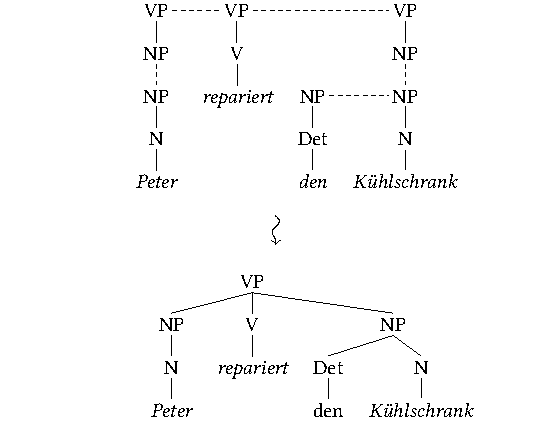
\includegraphics{graphics/abb91.pdf}
\caption{\label{fig-stug-1}Ableitung der syntaktischen Struktur von \ref{ex-stug-1} mittels Fusion und Substitution}
\end{figure}
Die horizontalen gestrichelten Linien deuten Fusionen an, die vertikalen gestrichelten Linien stehen für Substitutionen. Wie bei der Definition der Spinal-TT-MCTAG-Ableitungsbäume\is{TT-MCTAG!spinalisierte} (siehe Definition~\ref{def-spinal-ablbaum}, S.\,\pageref{def-spinal-ablbaum}) nehme ich im Folgenden die Einschränkung vor, dass nur \isi{Wurzelknoten} fusionieren können. Die \isi{Substitution} verwende ich in ihrer üblichen Form. Auf die Wurzeladjunktion, die noch bei Spinal-TT-MCTAG zum Einsatz kam, können wir hier verzichten, da die Lokalitätsbestimmung nicht von der Wahl der Verknüpfungsoperation abhängt. Das Konzept der Node-Sharing-Lokalität\is{Node Sharing} wird also ebenfalls nicht benötigt.

\largerpage%
Die \isi{Fusion} ist auf zweierlei Weise beschränkt: (i) Die fusionierende Knoten müssen ein identisches Label tragen und (ii) die Kette der Tochterknotenlabel muss in der Sprache desjenigen endlichen Automaten\is{endlicher Automat} sein, auf den das Label des Mutterknotens abgebildet wird. Der Fusionsbegriff wird also unverändert von Spinal-TT-MCTAG\is{TT-MCTAG!spinalisierte} übernommen (siehe Definition~\ref{def-fusion}, S.\,\pageref{def-fusion}).

\subsubsection*{Valenzstrukturen}\is{STUG!Valenzstruktur|(}

Einer syntaktischen Struktur wie in Abbildung~\ref{fig-stug-1} und den dort enthaltenen Elementarbäumen wird in einer STUG eine Valenzstruktur (bzw.\ eine Menge von Valenzstrukturfragmenten) zur Seite gestellt. Der Elementarbaum des finiten Verbs {\it repariert} ist dementsprechend das erste Element des 2-Tupels in Abbildung~\ref{fig-stug-2}, dessen zweites Element die Valenzstruktur darstellen soll.  
\begin{figure}[t]
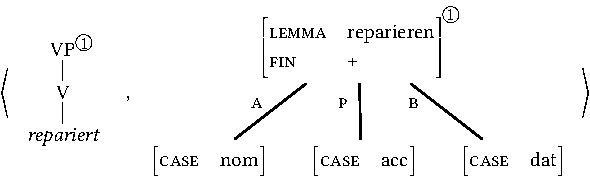
\includegraphics{graphics/abb92.pdf}
\caption{\label{fig-stug-2}STUG-Tupel für {\it repariert}}
\end{figure}
In dieser Arbeit schreibe ich die Valenzstruktur als Baum mit komplexen Knotenlabeln und atomaren Kantenlabeln auf, worin die Knoten für \isi{Valenzträger} bzw.\ Valenzrollen\is{semantische Rolle} stehen und die Kanten für Valenzbeziehungen\is{Valenzbeziehung}, die durch das Kantenlabel unterschieden werden. Der dominierende Knoten spezifiziert jeweils einen Valenzträger und seine Tochterknoten jeweils die dazugehörigen Valenzrollen. Die Valenzstruktur in Abbildung~\ref{fig-stug-2} bedeutet also, dass der Valenzträger drei Valenzrollen mit je unterschiedlichem Kasusmerkmal\is{Kasus} hat, wobei sich die Valenzbeziehungen entsprechend der Kantenlabel ({\sc a(gens), p(atiens), b(eneficans)}) unterscheiden.\footnote{Für den Ergänzungsstatus des benefikativen Dativs (bzw.\ des dativus commodi/incommodi) argumentiert z.\,B.\ \citet[115]{Wegener:85}.} Den folgenden Ausführungen lege ich ein funktionales Verständnis der Valenzbeziehungen\is{Valenzbeziehung} zugrunde, will sagen: Die von einem Mutterknoten ausgehenden Kanten haben paarweise verschiedene Label. Dieses funktionale Verständnis lie\ss e sich ohne Weiteres durch funktionale Merkmale einer Merkmalsstruktur formalisieren.\footnote{Die "`syntax-semantics interface representations"' aus \cite{Hahn:Meurers:11}, die dem Sinn und Zweck der Valenzstrukturen nahe kommen, sind zwar Merkmalsstrukturen, stellen die Valenz eines Valenzträgers allerdings als Liste von Ergänzungen dar. Dort müsste der funktionale Charakter der Valenzrollen also auch zusätzlich stipuliert werden.} Ich verwende hier jedoch eine Baumdarstellung, um auch Kantenlabel unterspezifizieren zu können (siehe z.\,B.\ Abbildung~\ref{fig-stug-3}).

STUG-Tupel enthalten mindestens einen Link zwischen einem Knoten der syntaktischen Struktur und einem Knoten der Valenzstruktur, annotiert mit den Linklabeln \circled{1} \ldots \circled{n}. In Abbildung~\ref{fig-stug-2} besteht ein solcher Link zwischen den Wurzelknoten der Tupel-Elemente. Bei der Verknüpfung zweier STUG-Tupel dürfen nur solche Valenzstrukturknoten mit Link unifiziert werden, die mit einem identischen syntaktischen Knoten verlinkt sind, also dasselbe Linklabel tragen. Dazu gleich mehr. 

Die für die Ableitung in Abbildung~\ref{fig-stug-1} au\ss erdem notwendigen STUG-Tupel für die nominalen Ergänzungen sind in Abbildung~\ref{fig-stug-3} aufgelistet.
\begin{figure}[t]
\centering
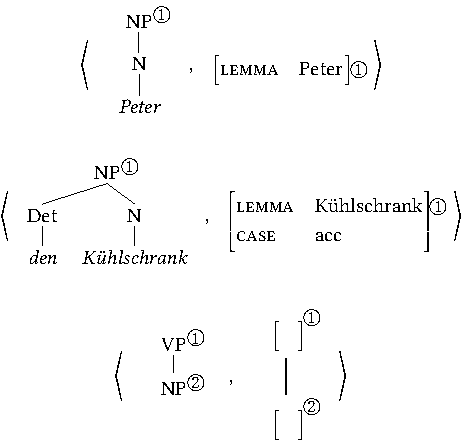
\includegraphics{graphics/abb93.pdf}
\caption{\label{fig-stug-3}Weitere elementare STUG-Tupel für die Derivation von \ref{ex-stug-1}}
\end{figure}
Da ich die NP-interne Syntax an dieser Stelle ausklammern möchte, ist {\it den Kühlschrank} als bereits abgeleitetes Tupel enthalten. Des weiteren simplifiziere ich die Valenzstruktur der Nomina, da uns in dieser Arbeit allein die Verbvalenz interessiert. Bei den STUG-Tupeln in Abbildung~\ref{fig-stug-3} sticht das letzte Tupel heraus, das für die Anknüpfung der NP-Konstituenten an den VP-Knoten benötigt wird. Seine Valenzstruktur besteht aus einer nicht weiter spezifizierte Valenzbeziehung, deren Valenzträger mit dem VP-Knoten und deren Valenzrolle mit dem NP-Knoten verlinkt sind.

\subsubsection*{Kombination von Valenzstrukturen}    

Wie werden nun die Valenzstrukturen der STUG-Tupel in Abbildung~\ref{fig-stug-2} und \ref{fig-stug-3} bei der Derivation der syntaktischen Struktur in Abbildung~\ref{fig-stug-1} kombiniert? Man kann einen Vereini\-gungs- und einen Unifikationsschritt unterscheiden. Abbildung~\ref{fig-stug-4} gibt dafür ein Beispiel: Werden zwei Syntaxbäume $\sigma_1$ und $\sigma_2$ per \isi{Fusion} oder Substitution zu $\sigma'$ verknüpft, dann werden die Tupel $\langle \sigma_1, V_1 \rangle$, $\langle \sigma_2, V_2 \rangle$ durch das Tupel $\langle \sigma', V_1 \cup V_2 \rangle$ ersetzt. Die Valenzstrukturen $V_1$ und $V_2$ werden also zunächst vereinigt, was darauf hindeutet, dass es sich beim zweiten Element eines STUG-Tupels eigentlich um eine Menge von Valenzstrukturen (bzw.\ Valenzstrukturfragmenten) handelt. Zur Vereinfachung der Darstellung der STUG-Tupel verzichte ich bei einelementigen Valenzstrukturmengen meist auf die Mengenklammer. Das Ergebnis dieses Vereinigungsschritts ist in Abbildung~\ref{fig-stug-4} im ersten Tupel wiedergegeben, wobei dort der Übersichtlichkeit halber die Valenzstrukturen der nominalen Ergänzungen bereits unifiziert wurden.
\begin{figure}[t]
\centering
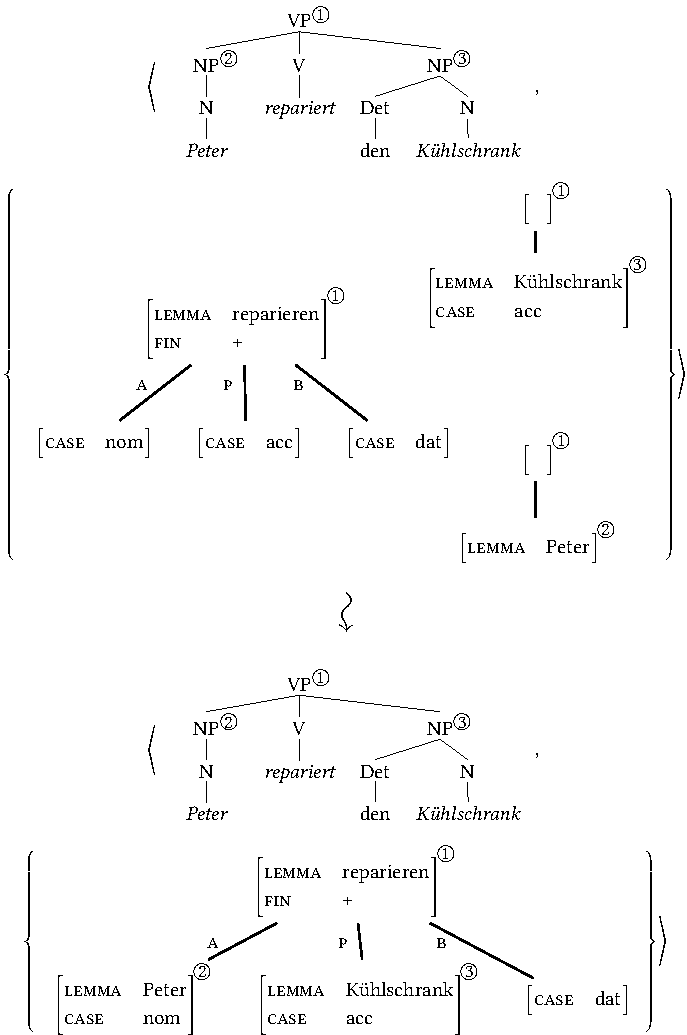
\includegraphics{graphics/abb94.pdf}
\caption{\label{fig-stug-4}STUG-Ableitung für \ref{ex-stug-1}}
\end{figure}

Wie man in Abbildung~\ref{fig-stug-4} au\ss erdem sehen kann, werden die Links beim Vereinigungsschritt übernommen: Die Links zu einem ersetzten Knoten beziehen sich danach auf den ersetzenden Knoten. Die Linklabel werden dabei so gewählt, dass zuvor unterschiedene Links auch nach der Vereinigung ein unterschiedliches Label tragen. 

Der Unifikationsschritt führt schlie\ss lich die Elemente der Valenzstrukturmenge zu einer zusammenhängenden Valenzstruktur zusammen. Unifizieren zwei Valenzstrukturen, so werden (unter Beibehaltung der jeweiligen Dominanzverhältnisse) beliebig viele ihrer Knoten und Kanten identifiziert und deren Label unifiziert. Die Unifikation von Valenzstrukturen operiert also auf ganzen Bäumen, wodurch sie sich wesentlich von der Wurzelknotenfusion in der syntaktischen Struktur, geschweige denn von der Verknüpfungsoperation bei STAG\is{Synchronous TAG (STAG)}, unterscheidet. Zwei STUG-spezifische Einschränkungen kommen bei der Valenzstrukturunifikation hinzu: (i) Valenzstrukturen können nur unifizieren, wenn dabei mindestens zwei Knoten unifiziert werden, die mit einem identischen Syntaxknoten verlinkt sind; (ii) Knoten mit Link können nur unifizieren, wenn sie mit einem identischen Syntaxknoten verlinkt sind. Damit wird die Unifizierbarkeit an die Zugehörigkeit zu einer syntaktischen Lokalitätsdomäne geknüpft. In Abbildung~\ref{fig-stug-4} ist ein mögliches Ergebnis des Unifikationsschrittes im zweiten Tupel zu sehen. Die Unifikation der {\it Peter}-Valenzstruktur mit der Agensrolle ist dabei keineswegs alternativlos -- sie könnte auch mit der Benefikans-Rolle unifizieren. Wie die Realisierung der Agensrolle erzwungen werden kann, werden wir weiter unten in Abschnitt \ref{sec-stug-ellipse} und \ref{sec-stug-vollst} sehen.

Wenn ich von Realisierung einer Valenzrolle spreche, dann meine ich die Spezifizierung des {\sc lemma}-Merkmals in einem Valenzrollenknoten. Man beachte, dass die {\sc lemma}-Spezifizie\-rung keine Bedingung für die Wohlgeformtheit einer Valenzstruktur darstellt. Valenzrollen und Valenzträger können beliebig unterspezifiert sein.
\is{STUG!Valenzstruktur|)}

\clearpage 

\subsubsection*{Kurzbeispiele: Passiv, Perfekt und Voranstellung}

Soweit die Darstellung der elementaren Wesenszüge des STUG"=Formalismus. Im Folgenden möchte ich, um einen besseren Eindruck der Modellierungswege zu vermitteln, die sich mit STUG eröffnen, kurz auf die passivische und die perfektivische Variante unseres Eingangsbeispiels in \ref{ex-stug-1} eingehen:

\ex. \label{ex-stug-2}
\a.  \label{ex-stug-2-a} Der Kühlschrank wird von Peter repariert.
\b. \label{ex-stug-2-b} Peter hat den Kühlschrank repariert.

Wenn wir von den STUG-Tupeln aus der obigen Fallstudie ausgehen, reicht die Hinzunahme der STUG-Tupel in Abbildung~\ref{fig-stug-5}, um den Sätzen in \ref{ex-stug-2} eine STUG-Analyse angedeihen zu lassen.
\begin{figure}[t]
\centering
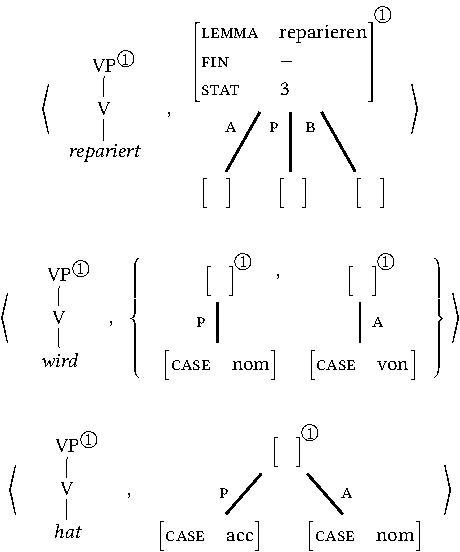
\includegraphics{graphics/abb95.pdf}
\caption{\label{fig-stug-5}Verbale STUG-Tupel für Passiv- und Perfektkonstruktionen}
\end{figure}
Das STUG-Tupel für das Partizip {\it repariert} unterscheidet sich von der finiten Variante (siehe Abbildung~\ref{fig-stug-2}) in den morphosyntaktischen Merkmalen im Wurzelknoten und dem Grad der Spezifizierung in den Valenzrollenknoten. Tatsächlich sind die Agens- und Patiensrolle vollkommen unspezifiziert. Diese Eigenschaft macht das {\it repariert}-Tupel sowohl für Passiv-\is{Passiv} als auch für Perfekt-Konstruktionen\is{Perfekt} verwendbar, indem die notwendige Spezifizierung durch das jeweilige \isi{Hilfsverb} beigesteuert wird. Dass dabei die Valenzrollen in getrennte Valenzstrukturfragmente aufgeteilt werden, hat in dem hier betrachteten Beispiel keine besondere Auswirkung. Bei der STUG-Analyse des Fernpassivs, auf die ich im nächsten Abschnitt eingehe, spielt das allerdings eine Rolle, da so die Valenzstrukturfragmente mit unterschiedlichen Valenzträgern unifizieren können.  

Als nächstes möchte ich den Blick auf die Modellierung partieller Voranstellungen\is{Voranstellung!partielle} wie der in \ref{ex-stug-3} lenken: 

\ex. \label{ex-stug-3}Der Kühlschrank repariert wird von Peter.

Für solche Fälle benötigt man ein spezielles unlexikalisiertes STUG-Tupel wie das in Abbildung~\ref{fig-stug-6}, das die \isi{Vorfeldbündelung} veranlasst. In der Valenzstruktur wird hier nur ein Knoten angenommen, der mit beiden Syntaxknoten verlinkt ist. Auf diese Weise können die beiden nominalen Ergänzungen {\it der Kühlschrank} und {\it von Peter} gleicherma\ss en mit dem Valenzträger {\it repariert} unifizieren.
\begin{figure}[t]
\centering
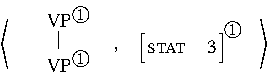
\includegraphics{graphics/abb96.pdf}
\caption{\label{fig-stug-6}Einbettendes STUG-Tupel für die Derivation der partiellen Voranstellung in \ref{ex-stug-3}}
\end{figure}
Die Einschränkung auf Status-3-Verben kann mittels eines morphosyntaktischen Merkmals in der Valenzstruktur vollzogen werden. Die Voranstellung von Status-2-Verben verlangt nämlich eine etwas andere Valenzstruktur nebst Verlinkung, wie wir gleich sehen werden. Ein Nachteil der Lösung in Abbildung~\ref{fig-stug-6} scheint jedoch in ihrer gro\ss en Permissivität zu liegen, da auch die unakzeptable Voranstellung\is{Voranstellung!partielle} mit \isi{Subjekt} in \ref{ex-stug-4-a} lizenziert wird:   

\ex. \label{ex-stug-4}
\a. *Peter gelesen hat den Roman. \hfill \citep[Abbildung~6]{Gerdes:04}\label{ex-stug-4-a}
\b. Ein Au\ss enseiter gewonnen hat hier noch nie. \hfill \citep[10-d]{Haider:90}\label{ex-stug-4-b}

\largerpage%
Andererseits ist gerade diese Permissivität für die Modellierung des vergleichbaren aber wesentlich akzeptableren Voranstellungsdatums in \ref{ex-stug-4-b} notwendig. Au\ss erdem wurde bei der Datendiskussion in Abschnitt~\ref{sec-kohaerenz-voran} vorsichtig vermutet, dass für die Unakzeptabilität von \ref{ex-stug-4-a} diskurs- und informationsstrukturelle Faktoren verantwortlich zu machen sind. Ich halte die Derivation von \ref{ex-stug-4-a} also für das kleinere Übel.

\subsubsection*{Desiderata}

Bevor eine erste Definition von STUG vorgenommen und danach auf die Modellierung kohärenter und elliptischer Konstruktionen eingegangen wird, möchte ich kurz auf zwei Desiderata hinweisen, nämlich die Modellierung von Angaben und die Modellierung der Stellungsvarianten im Verbalkomplex. Deren Klärung ist für ein umfassendes STUG-Modell des Deutschen sicherlich wichtig, aber keine Voraussetzung für den Fortlauf des Kapitels, da hier andere Phänomene im Fokus stehen.

Bisher wurden Valenzträger und Ergänzungen betrachtet, doch wie können Angaben\is{Angabe} in das STUG-Modell integriert werden? Folgt man dem klassischen Valenzbegriff aus Kapitel~\ref{ch-mit-valenz}, dann ist die Integration in die Valenzstruktur\is{STUG!Valenzstruktur} konzeptuell unangemessen, da sich Angaben ja gerade nicht in einer Valenzbeziehung zu einem Valenzträger befinden sollen. Ich schlage es aber trotzdem vor und berufe mich dabei auf einen Valenzbegriff, der sich an Storrers \isi{Situationsvalenz} orientiert und den ich in Abschnitt~\ref{sec-stug-implikationen} noch etwas genauer darstellen will. Angaben sollen also wie Ergänzungen als Valenzrollenknoten in der Valenzstruktur auf"|tauchen, wobei dann entsprechende Kantenlabel ({\sc t(empus)}, {\sc l(ocus)}, {\sc d(irectio)}, {\sc m(odus)}, \ldots) eingesetzt werden. Ein technisches Problem dieser Integration ist jedoch, dass der funktionale Charakter der Valenzrollen, der für Ergänzungen aus gutem Grund gelten soll, der \isi{Iterierbarkeit} von Angaben nicht gerecht wird:

\ex. \label{ex-stug-angabe} Am Freitag wollte Peter nach dem Abendessen den Kühlschrank reparieren.

Um Sätze wie \ref{ex-stug-angabe} mit iterierter Tempusbestimmung\is{Angabe} korrekt zu erfassen, kann man zu folgendem Trick greifen: Man verwendet doch komplexe Kantenlabel, bestehend aus einem Valenzrollenmerkmal und einem zweiten  Merkmal, z.\,B.\ einem Positionsmerkmal, das allerdings nur bei iterierbaren Valenzrollen spezifiziert ist. Dadurch unterscheiden sich die Kantenlabel aller iterierbaren Valenzrollen und müssen daher nicht unifiziert werden.      

Das zweite Desideratum betrifft die Wortstellung im \isi{Verbalkomplex}. Das dargestellte STUG-Modell unterscheidet nämlich nicht zwischen den beiden Stellungsvarianten in \ref{ex-stug-vkomplex}:

\ex. \label{ex-stug-vkomplex}
\a. dass Peter den Kühlschrank reparieren will 
\b. ?dass Peter den Kühlschrank will reparieren\label{ex-stug-vkomplex-b} 

Um bestimmte Stellungsvarianten wie die in \ref{ex-stug-vkomplex-b} zu blockieren, ohne die flache Phrasenstruktur\is{Phrasenstruktur!flache} aufzugeben, könnte man eine Indizierung des Verbalkomplex durchführen und den Positionsindex als morphologisches Merkmal in die Valenzstruktur\is{STUG!Valenzstruktur} übertragen. Das regierende Verb könnte dann auf diesen Positionsindex zugreifen und (mittels eines simplen Nachfolgeoperators) die korrekte Adjazenz sicherstellen. Ein solcher Mechanismus wäre auch nötig, um bei flacher Phrasenstruktur kreuzende Abhängigkeiten\is{kreuzende Abhängigkeit} im Niederländischen und Schweizerdeutschen korrekt zu analysieren und damit eines der MCS-Kriterien\is{schwache Kontextsensitivität} zu erfüllen.\footnote{Dies führt freilich dazu, dass die Menge der Knoten- und Kantenlabel unendlich ist.}


\subsection{Definitionen}\is{STUG!Definition|(}

Die STUG-Tupel bestehen aus einer syntaktischen Struktur und einer Menge von Valenzstrukturen. Die Unterschiede dieser Strukturtypen werden in folgenden Definitionen sichtbar:

\begin{definition}[Syntaktische Struktur] Sei $D = \langle E,V \rangle$ ein Baum. Eine syntaktische Struktur ist ein geordneter Baum $D_{\mathit{syn}} = \langle E,V,N,T,l_V \rangle$ mit einer Knotenlabelfunktion $l_V: V \to N\cup T$, wobei gilt:
\begin{itemize}
  \item $D_{\mathit{syn}}$ hat mindestens zwei Knoten.
  \item $N$, $T$ sind disjunkte Alphabete nicht-terminaler und terminaler Symbole.
  \item Wenn $l_v(v) \in T$, dann ist $v$ ein Blatt in $D$.
\end{itemize} 
\end{definition}

\is{STUG!Valenzstruktur}
\begin{definition}[Valenzstruktur]
Sei $D = \langle E,V \rangle$ ein Baum. Eine Valenzstruktur ist ein ungeordneter Baum $D_{\mathit{val}} = \langle E,V,F,W,l_V,R,l_E \rangle$ mit einer Knotenlabelfunktion $l_V : V \to 2^{F \times W}$ und einer Kantenlabelfunktion $l_E: E \to R$, wobei gilt:
\begin{itemize} 
  \item $l_V(v)$ für beliebiges $v \in V$ ist eine partielle Funktion $l_V(v): F \to W$, d.\,h.\ eine Menge von Merkmal-Wert-Paaren mit Merkmalen $F$ und Werten $W$.
  \item $R$ ist eine Menge von Valenzrollenkürzeln.
  \item Es gibt keine paarweise verschiedenen Knoten $v, v_i, v_j \in V$, so dass $((v,v_i),r)$ $\in l_E$ und $((v,v_j),r) \in l_E$ für beliebiges $r \in R$.
\end{itemize}  
\end{definition}
Syntaktische Strukturen sind linear geordnet, haben atomare Knotenlabel und keine Kantenlabel. Valenzstrukturen\is{STUG!Valenzstruktur} sind dagegen linear ungeordnet, verfügen über komplexe Knotenlabel in Form funktionaler Merkmalsstrukturen und über atomare Kantenlabel. Letztere sind in einer Valenzstruktur jedoch nicht beliebig verteilt, denn die von einem Knoten ausgehenden Kanten tragen paarweise verschiedene Kantenlabel.	

Basierend auf diesen Strukturtypen lässt sich die Form eines STUG-Tupels folgenderma\ss en definieren, wobei $P(A)$ eine Partition der Menge $A$ bedeutet soll:

\begin{definition}[STUG-Tupel]
Ein STUG-Tupel ist ein Tupel der Form $\langle \sigma,\{\phi_1,$\linebreak $\ldots,\phi_n\}, \frown\rangle$ bestehend aus einer syntaktischen Struktur $\sigma$, einer Menge von Valenzstrukturen $\{\phi_1,\ldots,\phi_n\}$ und einer Verlinkung $\frown$, für die gilt:
\begin{itemize}
  \item $\frown: P(V_\sigma) \to 2^{V_{\phi_1} \cup \ldots \cup V_{\phi_n}}$, wobei $V_\sigma$ die Knoten aus $\sigma$ und $V_{\phi_1}, \ldots, V_{\phi_n}$ die Knoten aus $\phi_1,\ldots,\phi_n$ sind.
  \item Für jedes $\phi_i \in \{\phi_1,\ldots,\phi_n\}$ mit Knoten $V_i$ existiert mindestens ein $\langle V_{\mathit{syn}},$ $V_{\mathit{val}}\rangle \in \ \frown$ mit $V_i \cap V_{\mathit{val}} \ne \emptyset$.
\end{itemize}
\end{definition}
Bemerkenswert an dieser STUG-Tupel-Definition ist sicherlich die Definition der Verlinkung, indem nämlich eine Partition von Syntaxknoten auf eine Potenzmenge von Valenzstrukturknoten abgebildet wird. Die Folge ist, dass die Syntaxknoten an maximal einer Verlinkung beteiligt sind, wogegen die Valenzstrukturknoten an beliebig vielen Verlinkungen beteiligt sein können. Die Mehrfachverlinkung kann z.\,B.\ bei der Modellierung der partiellen Voranstellung\is{Voranstellung!partielle} und der 3.~Konstruktion\is{kohärente Konstruktion!3.~Konstruktion} nötig sein (siehe Abbildung~\ref{fig-stug-10}, S.\,\pageref{fig-stug-10}).     

Diese Art der Verlinkung unterscheidet sich wesentlich von der Verlinkung in STAG\is{Synchronous TAG (STAG)}, die dort als Menge von Knotenpaaren definiert ist. Warum diese Abweichung? Eine Verlinkung mittels Knotenpaaren würde STUG nicht mit der nötigen Ausdrucksstärke ausstatten, z.\,B.\ um die partielle Voranstellung in \ref{ex-stug-7b} auf Seite~\pageref{ex-stug-7b} wie in Abbildung~\ref{fig-stug-13} auf Seite~\pageref{fig-stug-13} zu modellieren: Der vorangestellte eingebettete Valenzträger könnte dann nicht mit den Ergänzungen verknüpft werden, die im Mittelfeld der Matrix-VP platziert sind. Eine Verlinkung mittels Knotenmengenpaaren lässt dagegen die benötigte Flexibilität zu.   

Wiederum basierend auf den Definitionen für syntaktische Strukturen, Valenzstrukturen und STUG-Tupeln lässt sich eine STUG folgenderma\ss en definieren:

\begin{definition}[Synchronous TUG] Eine Synchronous Tree Unification Grammar ist ein Tupel
$STUG = \langle N,T, \Gamma_{\!\mathit{syn}}, \mathit{fsa} ,F ,W ,R ,\Gamma_{\!\mathit{val}}, \Gamma_{\!\mathit{stug}} \rangle$, wobei gilt:
\begin{itemize}
  \item $\Gamma_{\!\mathit{syn}}$ ist eine Menge elementarer syntaktischer Strukturen mit Knotenlabeln\linebreak $N \cup T$.
  \item $\mathit{fsa}: N \to M$ mit $M$ als der Menge der endlichen Automaten.
  \item $\Gamma_{\!\mathit{val}}$ ist eine Menge elementarer Valenzstrukturen mit Knotenlabeln aus $2^{F \times W}$ und den Kantenlabeln $R$.
  \item $\Gamma_{\!\mathit{stug}} \sqsubseteq \{\langle \sigma,\{\phi_1,\ldots,\phi_n\}, \frown\rangle \ | \ \sigma \in \Gamma_{\!\mathit{syn}} \ \wedge \ \phi_1,\ldots,\phi_n \in \Gamma_{\!\mathit{val}}\}$ sind elementare STUG-Tupel.  
\end{itemize}
\end{definition}
Entsprechend ihrer drei Teile werden die STUG-Tupel einer STUG in einem komplexen Ableitungsschritt kombiniert: Syntaktische Strukturen werden mittels \is{Substitution} und \is{Fusion} verknüpft, wobei die endlichen Automaten\is{endlicher Automat} in $\mathit{fsa}$ die Fusion regulieren (siehe Definition~\ref{def-fusion}, S.\,\pageref{def-fusion}); Valenzstrukturmengen werden vereinigt und die Verlinkungen (entsprechend der syntaktischen Verknüpfungsoperation) zusammengefügt:

\begin{definition}[STUG-Ableitungsschritt]
Seien $\langle \sigma_i, \phi_i, \frown_i \rangle$ und $\langle \sigma_j, \phi_j, \frown_j \rangle$ abgeleitete STUG-Tupel oder Instanzen elementarer STUG-Tupel. Entsteht durch Fusion oder Substitution von $\sigma_i$ und $\sigma_j$ eine syntaktische Struktur $\sigma_{ij}$, dann werden $\langle \sigma_i, \phi_i, \frown_i \rangle$ und $\langle \sigma_j, \phi_j, \frown_j \rangle$ durch $\langle \sigma_{ij}, \phi_i \cup \phi_j, \frown_{ij} \rangle$ ersetzt. 

Seien im Folgenden $v_i$ ein Knoten aus $\sigma_i$ und $v_j$ ein Knoten aus $\sigma_j$. Sei ferner $\langle V_{\mathit{syn}}^i, V_{\mathit{val}}^i \rangle \in \; \frown_i$ mit Knotenmengen $V_{\mathit{syn}}^i, V_{\mathit{val}}^i$ und $v_i \in V_{\mathit{syn}}^i$ und sei $\langle V_{\mathit{syn}}^j, V_{\mathit{val}}^j \rangle \in \; \frown_j$ mit Knotenmengen $V_{\mathit{syn}}^j, V_{\mathit{val}}^j$ und $v_j \in V_{\mathit{syn}}^j$:

\begin{itemize}
\item (\isi{Substitution}) Wird in $\sigma_{ij}$ $v_i$ durch $v_j$ ersetzt, dann gilt: \\
$\frown_{ij} \; = \; \frown_i \setminus \{\langle V_{\mathit{syn}}^i, V_{\mathit{val}}^i \rangle\} \; \cup \;\frown_j \setminus \{\langle V_{\mathit{syn}}^j, V_{\mathit{val}}^j \rangle\} \; \cup \; \{\langle V_{\mathit{syn}}^i \setminus \{v_i\} \; \cup \; V_{\mathit{syn}}^j \; , \; V_{\mathit{val}}^i \cup V_{\mathit{val}}^j \rangle\}$
\item (\isi{Fusion}) Werden in $\sigma_{ij}$ $v_i$ und $v_j$ durch $v_{ij}$ ersetzt, dann gilt: \\
$\frown_{ij} \; = \; \frown_i \setminus \{\langle V_{\mathit{syn}}^i, V_{\mathit{val}}^i \rangle\} \; \cup \; \frown_j \setminus \{\langle V_{\mathit{syn}}^j, V_{\mathit{val}}^j \rangle\} \; \cup \; \{\langle V_{\mathit{syn}}^i \setminus \{v_i\} \; \cup \; V_{\mathit{syn}}^j \setminus \{v_j\} \; \cup \; \{v_{ij}\} \; , \; V_{\mathit{val}}^i \cup V_{\mathit{val}}^j \rangle\}$
\end{itemize} 

\end{definition}   
Das Resultat dieses STUG-Ableitungsschritts ist also ein STUG-Tupel mit einer Menge von Valenzstrukturen, die zwar verlinkt, aber noch nicht unifiziert sind. Die Valenzstrukturunifikation ist tatsächlich von der STUG-Ableitung unabhängig und erfolgt in einem nachfolgenden Schritt. Um zu verstehen, was genau bei der Unifikation zweier Valenzstrukturen unifiziert, hilft das Konzept der isomorphen Teilbäume:  

\begin{definition}[Isomorphe Teilbäume]
Seien $D_i = \langle E_i,V_i \rangle$ und $D_j = \langle E_j,V_j \rangle$ Bäume.
Seien ferner $D_i' = \langle E_i', V_i' \rangle$ mit $E_i' \subseteq E_i$, $V_i' \subseteq V_i$ und $D_j' = \langle E_j', V_j' \rangle$ mit $E_j' \subseteq E_j$, $V_j' \subseteq V_j$ Teilbäume von $D_i$ und $D_j$. $D_i'$ und $D_j'$ sind isomorphe Teilbäume, falls es eine Bijektion $f:V_i' \to V_j'$ gibt, für die gilt: Falls $\langle v_{i1}', v_{i2}' \rangle \in E_i'$, dann $\langle f(v_{i1}'), f(v_{i2}') \rangle \in E_j'$.
\end{definition}
Die Valenzstrukturunifikation operiert auf folgende Weise auf den isomorphen Teilbäumen von Valenzstrukturen:\is{STUG!Valenzstruktur}

\begin{definition}[Valenzstrukturunifikation]
Seien $D_i = \langle E_i,V_i,F,V,l_{V\!\!\:i},R,l_{Ei} \rangle$\linebreak und $D_j = \langle E_j,V_j,F,V,l_{V\!j},R,l_{Ej} \rangle$ Valenzstrukturen. Seien $D_i' = \langle E_i', V_i' \rangle$ und $D_j' = \langle E_j', V_j' \rangle$ isomorphe Teilbäume von $D_i$ und $D_j$ dank der Bijektion $f:V_i' \to V_j'$.  Dann ist $D_{ij} = \langle E_{ij},V_{ij},F,V,l_{V\!\!\:ij},R,l_{Eij} \rangle$ das Ergebnis der Unifikation von $D_i$ und $D_j$, für das gilt:
\begin{itemize}
  \item $D_{ij}$ ist eine Valenzstruktur.
  \item $V_{ij} = V_i \cup V_j \setminus V_i'$
  \item $E_{ij} = E_i \cup E_j \setminus E_i' $\\
                 $~~~~~ \cup \ \{ (v, f(v_i')) \ | \ v_i' \in V_i' \ \wedge \ (v,v_i') \in E_i \setminus E_i' \}$ \\
                 $~~~~~ \cup \ \{ (f(v_i'),v) \ | \ v_i' \in V_i' \ \wedge \ (f(v_i'),v) \in E_i \setminus E_i'  \}$
  \item $l_{V\!\!\:ij} =  \{ (v,\mathit{fs}) \ | \ (v,\mathit{fs}) \in l_{V\!\!\:i} \ \wedge \ v \in V_i \setminus V_i' \} $ \\
                 $~~~~~ \cup \ \{ (v,\mathit{fs}) \ | \ (v,\mathit{fs}) \in l_{V\!j} \ \wedge \ v \in V_j \setminus V_j' \} $ \\
                 $~~~~~ \cup \ \{ (f(v),\mathit{fs}_i \cup \mathit{fs}_j) \ | \ (v,\mathit{fs}_i) \in l_{V\!\!\:i} \ \wedge \ v \in V_i' \ \wedge \ (f(v),\mathit{fs}_j) \in l_{V\!j} \ \wedge \ f(v) \in V_j' \} $ \\
                 für Merkmalsstrukturen $\mathit{fs}$, $\mathit{fs}_i$, $\mathit{fs}_j$.
  \item $l_{Eij} = \{ (e,r) \ | \ (e,r) \in l_{Ei} \ \wedge \ e \in E_i \setminus E_i' \} $ \\
                 $~~~~~ \cup \ \{ (e,r) \ | \ (e,r) \in l_{Ej} \ \wedge \ e \in E_j \setminus E_j' \} $ \\
                 $~~~~~ \cup \ \{ ((f(v_1),f(v_2)),r) \ | \  ((f(v_1),f(v_2)),r) \in l_{Ej} \ \vee \ ((v_1,v_2),r) \in l_{Ei} \ \wedge \  v_1,v_2 \in V_i'\} $ \\
                 für Vallenzrollenkürzel $r \in R$.                
\end{itemize}
\end{definition}
Dies ist die allgemeine Form der Valenzstrukturunifikation mit beliebigen isomorphen Teilbäumen. Dies berücksichtigt jedoch noch nicht die Verlinkung mit der syntaktischen Struktur. Dafür nehme ich folgende Einschränkung der betrachteten isomorphen Teilbäume vor: Sei $\langle \sigma, \Phi, \frown \rangle$ ein STUG-Tupel mit einem isomorphen Teilbaum $f$ von $\phi_i, \phi_j \in \Phi$. Unifizieren $\phi_i$ und $\phi_j$ anhand von $f$, dann gilt für $f$ zusätzlich:
\begin{itemize}
  \item Es gibt ein $\langle v_i,v_j \rangle \in f$ mit beliebigen Knoten $v_i,v_j$, so dass $v_i,v_j \in \; \frown\,(V_{\mathit{syn}})$ für beliebiges $V_{\mathit{syn}}$. Mit anderen Worten: Mindestens zwei miteinander unifizierende Valenzstrukturknoten sind mit demselben syntaktischen Knoten verlinkt.
  \item Falls $\langle v_i,v_j \rangle \in f$ mit beliebigen Knoten $v_i,v_j$ und $v_i \in \; \frown\,(V_{\mathit{syn}})$ für beliebiges $V_{\mathit{syn}}$ und $v_j \in \; \frown\,(V'_{\mathit{syn}})$ für beliebiges $V'_{\mathit{syn}}$, dann auch $v_i,v_j \in \; \frown\,(V''_{\mathit{syn}})$ für beliebiges $V''_{\mathit{syn}}$. Mit anderen Worten: Falls zwei miteinander unifizierende Valenzstrukturknoten mit einem syntaktischen Knoten verlinkt sind, dann sind sie auch mit einem identischen syntaktischen Knoten verlinkt.
  \item $f$ ist maximal gro\ss\ gewählt.
\end{itemize}

Eine vollständige STUG-Ableitung und Valenzstrukturunifikation resultiert in einem STUG-Tupel $\langle \sigma, \{\phi\}, \frown \rangle$ mit einer syntaktischen Struktur $\sigma$ ohne Blätter mit nicht-termina\-lem Knotenlabel und einer Valenzstruktur $\phi$.
\is{STUG!Definition|)}


\section{Modellierung kohärenter Konstruktionen} \label{sec-stug-kohaerenz}

Ausgehend von den STUG-Analysen im vorangegangenen Abschnitt möchte ich nun einen Modellierungsweg für kohärente Konstruktionen\is{kohärente Konstruktion} skizzieren. Wieder geht es darum, Potenzial und Eigenheit eines STUG-Modells zu veranschaulichen, ohne jedoch einen Detailgrad und einen empirischen Abdeckungsgrad wie z.\,B.\ bei der Darstellung des TT-MCTAG-Modells\is{TT-MCTAG} in Kapitel~\ref{sec-ttmctag} anzustreben. Stattdessen werde ich mich auf Konstruktionstypen beschränken, die sich im TT-MCTAG-Modell als besonders schwierig herausgestellt haben, nämlich das Fernpassiv und die mehrfach partielle Voranstellung.


\subsubsection*{Leichte Formen der Kohärenz}

Betrachten wir zunächst einen möglichst simplen Vertreter einer kohärenten Konstruktion: 

\ex. \label{ex-stug-5} Den Kühlschrank verspricht Peter zu reparieren.

Im Unterschied zu den oben behandelten Passiv- und Perfektkonstruktionen sind hier zwei verbale Valenzrahmen involviert, da nämlich {\it zu reparieren} als Valenzrolle seines Statusregens {\it verspricht} fungiert, während zugleich deren Valenzrollen relativ frei im Satz platziert werden können. Die Herausforderung besteht dann darin, sicherzustellen, dass die Valenzrollen von {\it zu reparieren} in der Valenzstruktur\is{STUG!Valenzstruktur} zum Valenzträger finden, auch wenn dieser, bezogen auf die syntaktische Lokalitätsdomäne, nicht den Wurzelknoten der Valenzstruktur bildet. Wie lässt sich dies in den STUG-Tupeln bewerkstelligen? In Abbildung~\ref{fig-stug-7} kann man sehen, dass dafür die Annahme eines weiteren Links im Regens {\it verspricht} ausreicht:
\begin{figure}[t]
\centering
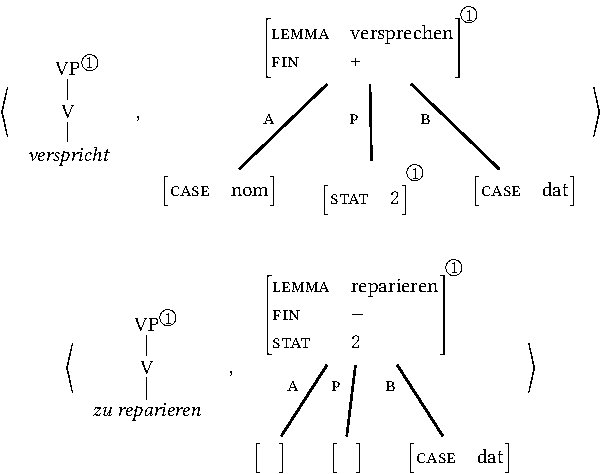
\includegraphics{graphics/abb97.pdf}
\caption{\label{fig-stug-7}STUG-Tupel für die Verben der kohärenten Konstruktion in \ref{ex-stug-5}}
\end{figure}
Indem nicht nur der Wurzelknoten, sondern auch der Valenzrollenknoten des regierten Verbs mit dem VP-Knoten verlinkt ist, können die nominalen Ergänzungen, die mit dem VP-Knoten fusionieren, auch auf letzteren zugreifen.  
Das Ergebnis der STUG-Derivation kann daher so aussehen wie in Abbildung~\ref{fig-stug-8}, wo {\it den Kühlschrank} als Valenzrolle des eingebetteten Verbs {\it zu reparieren} fungiert.
\begin{figure}[t]
\centering
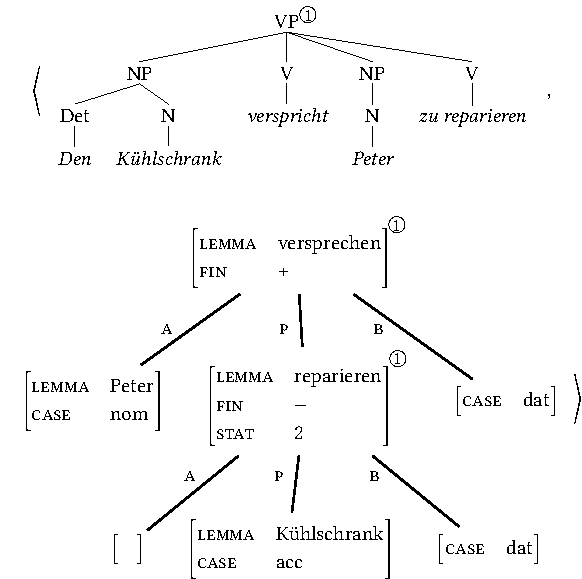
\includegraphics{graphics/abb98.pdf}
\caption{\label{fig-stug-8}Ergebnis der STUG-Derivation von \ref{ex-stug-5}}
\end{figure}

Natürlich ist das STUG-Tupel von {\it zu reparieren} in Abbildung~\ref{fig-stug-8} an sich viel zu permissiv, denn es verhindert beispielsweise nicht, alle drei Valenzrollen mit Dativ zu realisieren. Hier sind also entsprechende Kasusspezifikationen\is{Kasusmarkierung} (z.\,B.\ mittels Disjunktion im {\sc case}-Wert oder der Annahme mehrerer STUG-Tupel für {\it zu reparieren}) geboten, die ich aus Darstellungsgründen überspringe. Das gilt auch für Ma\ss nahmen, um zu verhindern, dass in beiden Valenzstrukturen (der von \textit{zu reparieren} und der von \textit{verspricht}) je ein Nominativ realisiert wird. Dafür könnte man ebenfalls spezielle Merkmale im Valenzträgerknoten von \textit{zu reparieren} annehmen, die helfen, die gewünschte Valenzstruktur aus dem Lexikon abzurufen. Auf zusätzliche Merkmale und entsprechende lexikalische Ambiguität kann aber möglicherweise verzichtet werden, wenn nämlich die Valenzstruktur von \textit{verspricht} direkt in die Valenzstruktur des regierten Infinitums eingreift und dort die Realisierung eines Nominativs unterbindet.   

\subsubsection*{Fernpassiv}\is{Passiv!Fern-|(}

Die im vorangegangenen Abschnitt bereits erläuterte Modellierung des Passivs kann unverändert auf kohärente Konstruktionen angewandt werden, wobei en passant auch die Fernpassiv-Konstruktion in \ref{ex-stug-7} korrekt erfasst wird:

\ex. \label{ex-stug-7} Der Kühlschrank wird von Peter zu reparieren versprochen.

Die dafür benötigten verbalen STUG-Tupel werden in Abbildung~\ref{fig-stug-11} aufgelistet.
\begin{figure}[t]
\centering
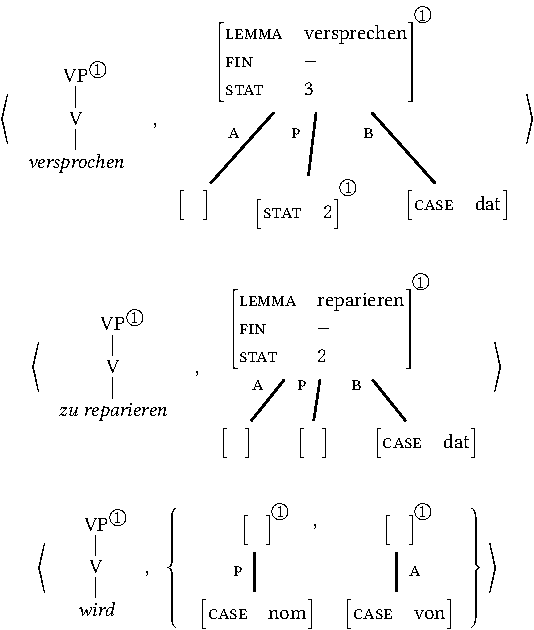
\includegraphics{graphics/abb99.pdf}
\caption{\label{fig-stug-11}Elementare verbale STUG-Tupel für die Derivation des Fernpassivs in \ref{ex-stug-7}}
\end{figure} 
Die Valenzstruktur von {\it versprochen} entspricht im Wesentlichen der Form anderer Status-3-Verben. Der Eintrag für das Passivhilfsverb ist ebenfalls bereits bekannt aus Abbildung~\ref{fig-stug-5}. Die Valenzstrukturfragmente spezifizieren zwei Valenzbeziehungen zwischen einem noch unbekannten Valenzträger und einer nominalen Konstitutente, nämlich einer Nominativ-NP einerseits und einer \emph{von}-PP andererseits. Damit gelangen wir für Satz \ref{ex-stug-7} zu dem abgeleiteten STUG-Tupel in Abbildung~\ref{fig-stug-12}.
\begin{figure}[t]
\centering
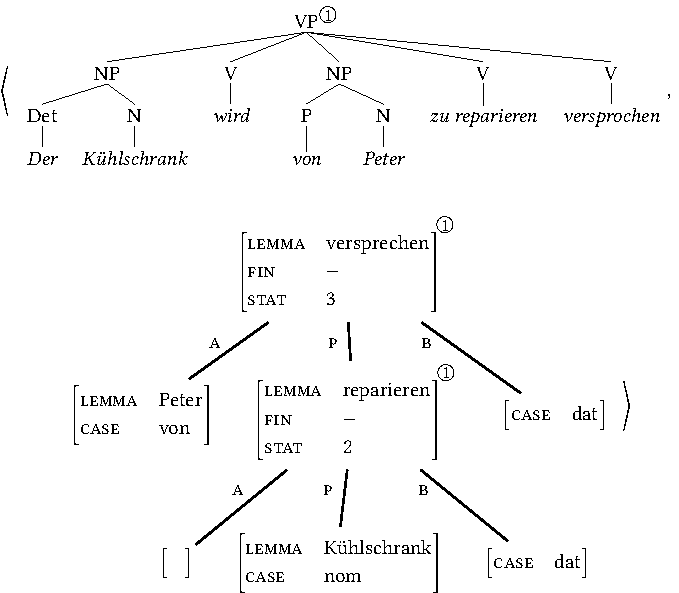
\includegraphics{graphics/abb910.pdf}
\caption{\label{fig-stug-12} Ergebnis der STUG-Derivation des Fernpassivs in \ref{ex-stug-7}}
\end{figure}
Dort erscheint das Fernpassiv in Gestalt der Nominativspezifizierung der Patiensrolle des eingebetteten Status-2-Verbs, die auf das Passivhilfsverb zurückgeht und durch die bei kohärenten Kontruktionen vorhandene Verlinkung ermöglicht wird.
\is{Passiv!Fern-|)} 

\subsubsection*{3.~Konstruktion und partielle Voranstellung}\is{kohärente Konstruktion!3.~Konstruktion|(}\is{Voranstellung!partielle|(}

Meint man, die Frage beantwortet zu haben, wie die Ergänzungen unterschiedlicher Verben in einer gemeinsamen syntaktischen Domäne permutieren können, so stellt sich gleich die nächste: Wie lässt sich dann das Nebeneinander kohärenter und inkohärenter Bereiche in der 3.~Konstruktion und der partiellen Voranstellung korrekt erfassen? Gemeint sind damit Daten wie in \ref{ex-stug-6}:

\ex. \label{ex-stug-6}
\a. \label{ex-stug-6-a} dass er den Kühlschrank verspricht, zu reparieren.
\b. \label{ex-stug-6-b} Zu reparieren verspricht er den Kühlschrank.

Die Antwort fällt wieder relativ kurz aus. Zwar ist es mit einem weiteren Link nicht getan, aber bereits die zusätzliche Annahme des STUG-Tupels in Abbildung~\ref{fig-stug-9} sorgt für die gewünschten Effekte.
\begin{figure}[t]
\centering
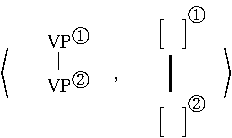
\includegraphics{graphics/abb911.pdf}
\caption{\label{fig-stug-9}Einbettendes STUG-Tupel für partielle Voranstellungen und die 3. Konstruktion}
\end{figure}
Dieses unlexikalisierte STUG-Tupel unterscheidet zwei in einem Dominanzverhältnis befindlichen VP-Domänen, die analog mit Mutter und Tochter einer Valenzbeziehung verlinkt sind. Man beachte, dass solch ein unlexikalisiertes STUG-Tupel in Fällen komplexer Voranstellung dann verwendet werden muss, wenn die endlichen Automaten der Fusionsregulierung eine Vorfeldbündelung vorsehen (vgl.\ Abbildung~\ref{fig-fsa}, S.\,\pageref{fig-fsa}). In Kombination mit den STUG-Tupeln in Abbildung~\ref{fig-stug-7} ergibt sich dann etwa für Satz \ref{ex-stug-6-b} das abgeleitete STUG-Tupel in Abbildung~\ref{fig-stug-10}.
\begin{figure}[t]
\centering
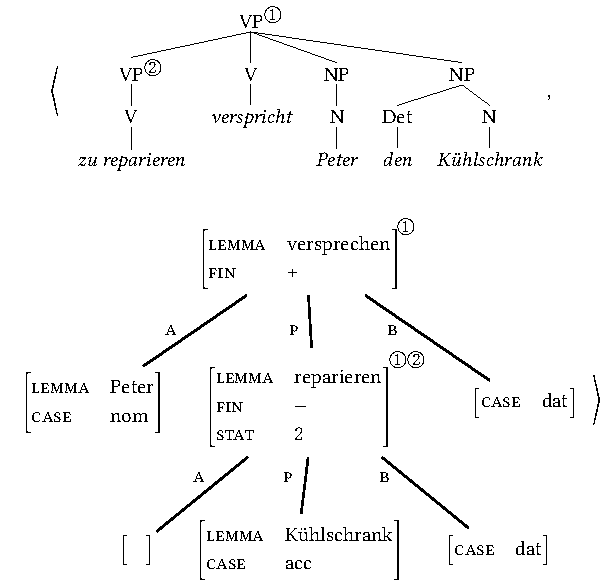
\includegraphics{graphics/abb912.pdf}
\caption{\label{fig-stug-10} Abgeleitetes STUG-Tupel für die partielle Voranstellung in \ref{ex-stug-6-b}}
\end{figure}
\largerpage%
Durch die Verlinkung des VP-Wurzelknotens mit dem {\it reparieren}-Knoten in der Valenzstruktur kann {\it den Kühlschrank}, eine Konstituente des Mittelfelds, auf diesen zugreifen. {\it den Kühlschrank} könnte jedoch auch mit einer Valenzrolle des Regens unifizieren. Im Unterschied dazu ist die Vorfeld-VP nur mit dem {\it reparieren}-Knoten verlinkt und nicht mit seinem Regens, d.\,h.\ mit dem Wurzelknoten der Valenzstruktur. Dadurch können Elemente, die mit der Vorfeld-VP fusionieren nicht auf den Valenzstrukturknoten des Regens zugreifen und die gewünschte Asymmetrie entsteht. Da sich das einbettende STUG-Tupel in Abbildung~\ref{fig-stug-9} auch bei der Modellierung der 3.~Konstruktion einsetzen lässt, ergeben sich dort ebenfalls die gewünschten Asymmetrieeffekte. 
\is{kohärente Konstruktion!3.~Konstruktion|)}
\largerpage%

\subsubsection*{Mehrfach partielle Voranstellung}

Von der einfachen partiellen Voranstellung in \ref{ex-stug-6-b} ist es im STUG-Modell nicht mehr weit bis zur mehrfach partiellen Voranstellung in \ref{ex-stug-7b}, die sich in Kapitel~\ref{sec-ttmctag} als besondere Herausforderung für die TT-MCTAG-Modellierung herausgestellt hat:  

\ex. \label{ex-stug-7b} Zu reparieren versprochen hat ihm das Peter.

Die für die Derivation von \ref{ex-stug-7b} nötigen verbalen STUG-Tupel fanden bereits in anderen Beispielen Verwendung. In Abbildung~\ref{fig-stug-13} werden sie nochmals dargestellt, neben dem Resultat der STUG-Derivation.   
\begin{figure}[t]
\centering
\resizebox{!}{0.9\textheight}{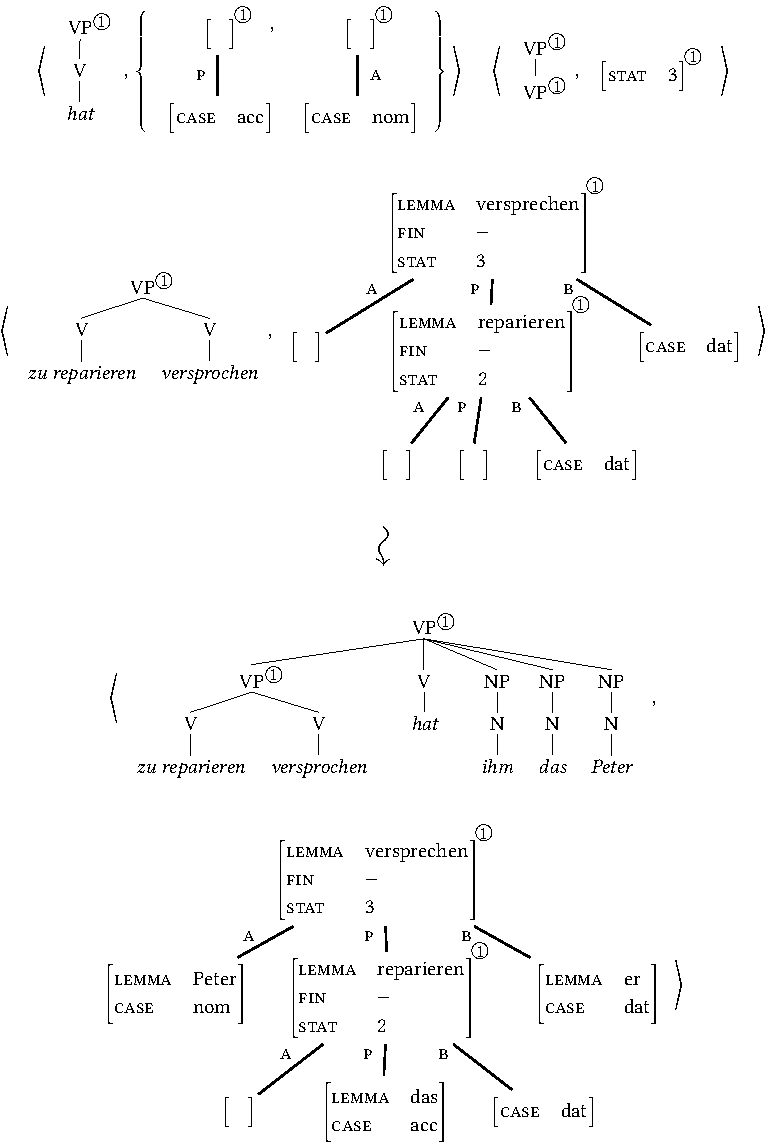
\includegraphics{graphics/abb913.pdf}}
\caption{\label{fig-stug-13} STUG-Ableitung der mehrfach partiellen Voranstellung in \ref{ex-stug-7b}}
\end{figure}
Das zweite STUG-Tupel dient der Voranstellung von VPs mit partizipialem Kopf, wobei die Verlinkung beider VP-Knoten im Zusammenspiel mit dem Verlinkungsmuster bei kohärenten Verben das Mittelfeld für Ergänzungen des eingebettet vorangestellten Verbs {\it zu reparieren} zugänglich macht. {\it Zu reparieren} selber ist in Abbildung~\ref{fig-stug-13} Teil des dritten STUG-Tupels, das bereits aus elementaren STUG-Tupeln abgeleitet wurde. Der angesichts solcher Datentypen bei der TT-MCTAG-Modellierung festgestellte Bedarf zur Erweiterung der Node-Sharing-Lokalität (zur Tree-Sharing-Lokalität) stellt sich bei STUG aufgrund der flachen Phrasenstruktur\is{Phrasenstruktur!flache} nicht ein. Ein Lokalitätsdomäne kann hier an einzelne Knoten festgemacht werden, während bei TT-MCTAG eine Lokalitätsdomäne eine variable Menge von Knoten umfassen muss. Dieses meiner Ansicht nach wünschenswerte Merkmal hat STUG mit Spinal-TT-MCTAG gemein und ist sicherlich mit der Verfügbarkeit der Fusions"=Operation zu erklären.\is{Voranstellung!partielle|)}%\\ 

Es sollte deutlich geworden sein, dass und wie Diskontinuitäten im Rahmen kohärenter Konstruktionen mit einer STUG modelliert werden können. Im Folgenden werde ich abschlie\ss end zwei Desiderata aufgreifen, auf deren Klärung hin das skizzierte STUG-Modell weiterentwickelt werden muss.

\subsubsection*{Desiderata}

Das bis hierhin dargelegte STUG-Modell kann die als unakzeptabel eingestufte Verteilung der Rektionskettenglieder in \ref{ex-stug-8} nicht verhindern:

\ex. \label{ex-stug-8}
\a. ?Versprochen hat ihm das Peter zu reparieren.\label{ex-stug-8-a}
\b. *Müssen wird er ihr ein Märchen erzählen. \hfill (\ref{ex-mueller-243}, S.\,\pageref{ex-mueller-243})\label{ex-stug-8-b}

Der Grund für die Unakzeptabilität dieser Sätze ist wohl, dass die vorangestellten\is{Voranstellung!partielle} Verben {\it versprochen} und {\it müssen} jeweils ein Verb in der rechten Satzklammer regieren, nämlich {\it zu reparieren} bzw.\ {\it erzählen} (siehe Abschnitt~\ref{sec-kohaerenz-voran}). Linearisierungssyntaktisch betrachtet sind diese Sätze jedoch unauf"|fällig und mit den oben eingeführten STUG-Tupeln lässt sich auch ohne Weiteres eine adäquate Valenzstruktur errechnen. Mit anderen Worten: Das STUG-Modell scheint an dieser Stelle zu permissiv zu sein. In meinen Augen liegt der Schlüssel für eine angemessene Beschränkung in der Ausarbeitung der Verbalkomplexsyntax\is{Verbalkomplex}. Würde nämlich das vorangestellte Regens das regierte Verb im vorangestellten Verbalkomplex erwarten, dann könnte für solche Sätze wie in \ref{ex-stug-8} keine verbundene Valenzstruktur gebildet werden, denn das regierte Verb entspräche dann nicht den spezifischen morphosyntaktischen Merkmalen einer Valenzrolle des Regens. Dieser Ansatz würde also vorhersagen, dass Sätze wie \ref{ex-stug-8} kein Verbalkomplex in der rechten \isi{Satzklammer} haben können. Während in \ref{ex-stug-8-a} dann noch eine alternative Analyse als 3.~Konstruktion denkbar wäre, ist das in \ref{ex-stug-8-b} ausgeschlossen. 

Die Platzierung des statusregierten Verbs spielt auch bei obligatorisch kohärent konstruierenden Verben\is{Kohärenz!obligatorische/fakultative} wie {\it müssen} und {\it scheinen} eine Rolle, denn das statusregierte Verb kann hier zwar vorangestellt aber nicht nachgestellt werden:

\ex.
\a. *dass er den Wagen muss ohne Werkzeug reparieren \hfill (\ref{ex-3konstr-modal-a}, S.\,\pageref{ex-3konstr-modal-a})
\b. *dass er ohne Werkzeug scheint, den Wagen zu reparieren \hfill (\ref{ex-3konstr-scheinen}, S.\,\pageref{ex-3konstr-scheinen})

Diese Form der Asymmetrie lässt sich auf zweierlei Weise modellieren: Zum einen kann schon bei der Fusion die Nachstellung (d.\,h.\ die Platzierung im Nachfeld) von Status-1-VPs blockiert werden; zum anderen kann eine entsprechende Einschränkung in der Valenzstruktur spezifiziert werden, falls felderspezifische Positionsmerkmale dort verfügbar sind. Letzteres würde insbesondere bei einem obligatorisch kohärenten Verb wie {\it scheinen}, das den 2.~Status regiert, in Frage kommen.

\clearpage

% Wie verhindern? Status-1-VPs können nicht im Nachfeld stehen!

Das zweite Desideratum ist die Modellierung sogenannter Brückenkonstruktionen\is{Brückenkonstruktion}. Dabei handelt es sich um  Fälle langer Extraktion aus Komplementsätzen\is{Komplementsatz} wie beispielsweise in \ref{ex-stug-9}: 

\ex. \label{ex-stug-9} Wen glaubst du, dass er repariert hat?

Hier wurde, der Bewegungsmetapher folgend, die W-Phrase aus dem \textit{dass}-Satz\is{Satz!\textit{dass}-} extrahiert, was zunächst nur bedeuten soll, dass die W-Phrase eine Ergänzung des im \emph{dass}-Satz eingebetteten Verbs {\it repariert} ist. Brückenkonstruktionen sind zum einen auf bestimmte Verben und Komplementsatztypen beschränkt und zum anderen kann die \isi{Extraktion} nur auf bestimmte Positionen im Matrixsatz abzielen, nämlich grob gesagt auf das Vorfeld (\citealt[Abschnitt~4.2.1.2]{Kvam:83}; \citealt{Luehr:88}; \citealt[Abschnitt~1.2]{Lutz:04}):\footnote{Im Framework der Generativen Grammatik wird lange Bewegung durch das Subjazenzprinzip (\citealt{Chomsky:73}; \citealt[Kapitel~6]{Chomsky:86}) eingeschränkt. Es besagt ungefähr, dass lange Bewegungen\is{Bewegung} bestimmte Knoten, etwa SpecC, nicht kreuzen können, ohne dort eine \isi{Spur} zu hinterlassen. Sie verlaufen also zyklisch, d.\,h.\ in Etappen. Das Subjazenzprinzip allein verhindert aber nicht lange Extraktionen ins Mittelfeld, die die Sätze in \ref{ex-stug-9-bc} ungrammatisch machen. Siehe G.\,\cite{Mueller:Sternefeld:93}.}

\ex. \label{ex-stug-9-bc}
\a. ??Du glaubst wen, dass er repariert hat?\label{ex-stug-9-b} 
\b. *\ldots\ dass du wen glaubst, dass er repariert hat?\label{ex-stug-9-c} 

\textit{Dass}-Sätze konstituieren also gewissermaßen Bewegungshalbinseln\is{Bewegungsinsel} und die Herausforderung besteht darin, diese Bewegungshalbinseln nur den nötigen Spalt zu öffnen, ohne eine massive Übergenerierung zu verursachen. Zu den Stärken von TAG zählt, dies auf relativ simple und dennoch kontrollierte Weise zu bewerkstelligen \citep{Kroch:89,Frank:06}. Dagegen scheint mir das bis hierhin dargelegte STUG-Modell entweder zu restriktiv oder zu permissiv zu sein. Zu restriktiv ist es, wenn man \textit{dass}-Sätze wie gewöhnliche NP-Komplemente behandelt, und zu permissiv, wenn man stattdessen \textit{dass}-Sätze wie Infinitiv-VPs in der 3.~Konstruktion analysiert. Es ist aber noch nicht vollständig geklärt, ob ein Zwischenweg mit den vorhandenen Mitteln nicht doch möglich ist. Andernfalls könnte ein Konstruktionsmodul weiterhelfen, das in der Lage wäre, die Verlinkung bei der STUG-Analyse von \ref{ex-stug-9} rekursiv so zu modifizieren, dass die Valenzstruktur von {\it wen} direkt mit der Valenzstruktur des eingebetteten \emph{dass}-Satzes unifiziert. In die Zuständigkeit des Konstruktionsmoduls würden übrigens nicht zwingend idiomatische Mehrwortausdrücke\is{Mehrwortausdruck} wie {\it Bauklötze staunen} fallen, denn hierfür reicht die Lokalitätsdomäne der Valenzstruktur\is{STUG!Valenzstruktur} prinzipiell aus.


\section{Modellierung elliptischer Strukturen} \label{sec-stug-ellipse}

Nachdem im letzten Abschnitt die Mächtigkeit des STUG-Formalismus hinsichtlich der direkten Repräsentation diskontinuierlicher Valenzrahmenrealisierungen demonstriert wurde, kreist dieser Abschnitt um das Potential des STUG-Formalismus, genuin unvollständige Strukturen\is{Unvollständigkeit!genuine} zu erzeugen und damit einen neuartigen Weg der Ellipsenmodellierung zu beschreiten. Dabei beschränke ich mich auf die STUG-Modellierung der Gappingregeln G1--G3\is{Gappingregel}, die in Kapitel~\ref{chap-ellipse} herausgearbeitet wurden. 

%\subsubsection*{Gappingregel G1}%
\is{Gappingregel!G1|(}

Die Gappingregel G1 besagt, dass die Ellipse immer das finite Verb umfasst -- so wie in der Koordinationsellipse\is{Ellipse!Koordinations-} in \ref{ex-stug-10}:

\ex. \label{ex-stug-10} [$\kappa_1$ Susi repariert das Auto] und [$\kappa_2$ Peter \sout{repariert} den Kühlschrank]. 

Die STUG-Derivation von $\kappa_2$ benötigt keine leeren Elemente\is{leere Kategorie} oder spezielle Elementarstrukturen, um das fehlende Verb zu kompensieren. Die nominalen Überbleibsel werden einfach per \isi{Fusion} verknüpft und deren Valenzstrukturen entsprechend unifiziert. Heraus kommt das STUG-Tupel in Abbildung~\ref{fig-stug-14}. 
\begin{figure}[t]
\centering
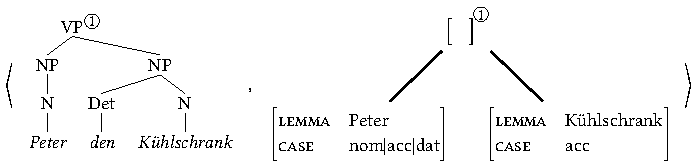
\includegraphics{graphics/abb914.pdf}
\caption{\label{fig-stug-14} Ergebnis der STUG-Derivation der Gappingkonstruktion in \ref{ex-stug-10}}
\end{figure}
Die Abwesenheit eines finiten Verbs führt also schlimmstenfalls zu einem unspezifizierten Valenzträgerknoten in der Valenzstruktur\is{STUG!Valenzstruktur}, dessen Spezifizierung Aufgabe eines hier nicht weiter ausgeführten Rekonstruktionsmechanismus\is{Rekonstruktion} ist. 

Da aber weder die syntaktische Struktur noch die Valenzstruktur irgendeinen Begriff von Vollständigkeit haben, stellt sich natürlich die Frage, wie man der Unakzeptabilität von \ref{ex-stug-11} gerecht werden kann:

\ex. \label{ex-stug-11} *Den Kühlschrank repariert \sout{Peter}.

In Widerspruch zu G1 umfasst hier die Ellipse zwar die obligatorische Nominativ"=Ergänzung\is{Ergänzung!obligatorische} aber nicht den finiten Valenzträger {\it repariert}. Das STUG-Modell muss also den Zusammenhang zwischen finitem Verb und der Realisierung bestimmter Valenzrollen irgendwie herstellen. Der richtige Ort dafür scheint mir die Valenzstruktur des finiten Verbs zu sein, wo die obligatorischen Ergänzungen als solche markiert werden. Das ist in Abbildung~\ref{fig-stug-15} mit dem Ausrufezeichen geschehen, das eine Spezifizierungspflicht für das {\sc lemma}-Merkmal ausdrücken soll.
\begin{figure}[t]
\centering
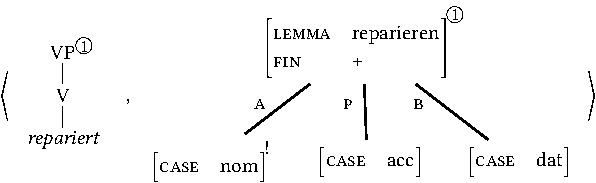
\includegraphics{graphics/abb915.pdf}
\caption{\label{fig-stug-15}STUG-Tupel für {\it repariert} mit !-Markierung an der obligatorischen Nominativ-Valenzrolle}
\end{figure}
Während noch offen ist, wie diese Markierung im STUG-Formalismus implementiert werden kann, wird also bereits deutlich, dass die Unakzeptabilität von Daten wie \ref{ex-stug-11} auf Eigenschaften ihrer Valenzstruktur zurückgeführt wird und nicht mit ihrer syntaktischen Struktur zusammenhängen soll. Was es mit dieser Differenzierung auf sich hat, werde ich in Abschnitt~\ref{sec-stug-vollst} skizzieren. 
\is{Gappingregel!G1|)}

%\subsubsection*{Gappingregel G2$^+$}%
\label{sec-stug-g2}\is{Gappingregel!G2$^+$|(}

Gemä\ss\ der Gappingregel G2$^+$ haben die Überbleibsel einer Ellipse immer den Umfang vollständiger Satzglieder\is{Satzglied}, wobei Teilsätze davon ausgenommen werden. G2$^+$ erfasst zunächst einmal korrekt die Unakzeptabilität von \ref{ex-stug-12}: 

\ex. \label{ex-stug-12} *[$\kappa_1$ Sven lebt in Mainz] und [$\kappa_2$ Stefan \sout{lebt in} Karlsruhe]. 

In der STUG-Derivation für \ref{ex-stug-12} würde zunächst nichts darauf hinweisen und wir erhielten für das zweite Konjunkt die Valenzstruktur in Abbildung~\ref{fig-stug-16}. 
\begin{figure}[t]
\centering
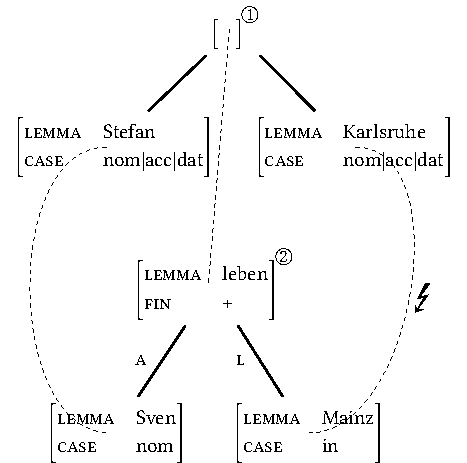
\includegraphics{graphics/abb916.pdf}
\caption{\label{fig-stug-16}Ellipse-Antezedens-Relationen (gestrichelte Linien) zwischen den Valenzstrukturen der Konjunkte in \ref{ex-stug-12}}
\end{figure}
Ein Problem entstünde allerdings bei der \isi{Rekonstruktion} des Valenzträgerknotens aus dem ersten Konjunkt. Sollte hierbei eine weitgehende Parallelität von Ellipse und Antezedens hinsichtlich der Valenzstruktur\is{STUG!Valenzstruktur} herrschen und daher der Valenzträger des Antezendens mit dem Valenzträger der Ellipse identisch sein, dann ergäbe sich in \ref{ex-stug-12} folgendes Problem: Da {\it lebt} nur Valenzrollen für eine Nominativ-NP und eine PP mit lokaler Präposition bereithält, könnte es mit der Valenzstruktur des zweiten Konjunkts nicht unifizieren. Dieser Sichtweise zufolge ist G2$^+$ also eine Folgeerscheinung des Rekonstruktionsmechanismus.  

Dass der Rekonstruktionsmechanismus, ohne auf ihn an dieser Stelle im Detail einzugehen, auch mit strukturell wesentlich komplexeren Fällen als \ref{ex-stug-12} zurecht kommen muss, offenbart ein Blick auf valenzrahmenübergreifendes Gapping wie in \ref{ex-stug-13}:

\ex. \label{ex-stug-13} [$\kappa_1$ Susi verspricht das Auto zu reparieren] und [$\kappa_2$ Peter \sout{verspricht} den Kühlschrank \sout{zu reparieren}].

Wenn wir für die Konjunkte in \ref{ex-stug-13} die Valenzstrukturen in Abbildung~\ref{fig-stug-17} als Grundlage hernehmen, dann müssen im Rahmen der \isi{Rekonstruktion} (wie in der Abbildung angedeutet) die folgenden Korrelationen etabliert werden: Der leere Valenzträgerknoten der Ellipse korreliert mit zwei Valenzträgerknoten im Antezedens und die Valenzrollenknoten der Ellipse korrelieren mit Valenzrollenknoten unterschiedlicher Valenzträger.
\begin{figure}[t]
\centering
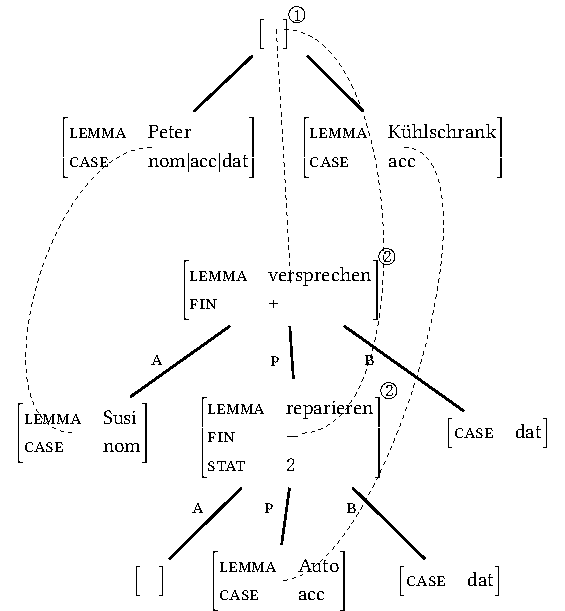
\includegraphics{graphics/abb917.pdf}
\caption{\label{fig-stug-17}Valenzstrukturen für die Konjunkte in \ref{ex-stug-13} mit den zu rekonstruierenden Ellipse-Antezedens-Relationen}
\end{figure}
Die Implementierung eines solch mächtigen Rekonstruktionsmechanismus kann sich möglicherweise an der Higher Order Unification für Lambda-Ausdrücke orientieren, die oben in Abschnitt~\ref{sec-fuellung} (S.\,\pageref{ex-fuellung-4}) erwähnt wurde. In dieser Hinsicht besteht also eine gewissen Ähnlichkeit zu unstrukturierten Füllungen\is{Füllung!unstrukturierte}, die ja ebenfalls mit mehreren Antezedensknoten in Beziehung stehen können. 
\is{Gappingregel!G2$^+$|)}

%\subsubsection*{Gappingregel G3}%
\is{Gappingregel!G3|(}

Die Gappingregel G3 fordert die Realisierung des finiten Verbs in Teilsätzen mit \emph{dass}-Kom\-ple\-mentierer\is{Komplementierer} und trägt damit der Unakzeptabilität von \ref{ex-stug-14} Rechnung:  

\ex. \label{ex-stug-14} *Peter verspricht, dass den Kühlschrank.

Da hier nur die Kookkurrenz zweier morphologisch charakterisierter Konstituenten gefordert wird, kann sich die STUG-Implementierung von G3 auf die Derivation der syntaktischen Struktur beschränken, indem z.\,B.\ die Fusionsmöglichkeiten von VP-Knoten mit einem endlichen Automaten\is{endlicher Automat} wie in Abbildung~\ref{fig-stug-18} geregelt werden. Damit unterscheidet sich die Implementierung von G3 wesentlich von den Implementierungen der anderen Gappingregeln, die auf der Valenzstruktur operieren.
\begin{figure}[t]
\centering
\begin{tikzpicture}[->,>=stealth',shorten >=1pt,auto,node distance=2.8cm,
                    semithick]
  \tikzstyle{every state}=[draw=black,text=black]

  \node[initial,initial text={},state] (A) {$z_0$};
  \node[state]         (B) [right of=A]   {$z_1$};
  \node[state,accepting]         (C) [right of=B]    {$z_2$};

  \path (A) edge node {\textit{dass}} (B)
        (B) edge [loop above] node {\textsc{ap|np|vp}} (C)
            edge node {\textsc{v}$_{\text{fin}}$} (C)
        ;
\end{tikzpicture}
\caption{\label{fig-stug-18}Endlicher Automat für die Fusion von VP-Knoten, der die Derivation des unvollständigen \emph{dass}-Teilsatzes in \ref{ex-stug-14} verhindert}
\end{figure}
\is{Gappingregel!G3|)}



\section{Anknüpfungspunkte in der Literatur} \label{sec-stug-implikationen}

Das vorgestellte STUG-Modell implementiert nicht neuartige grammatiktheoretische Ideen, sondern es schafft und konkretisiert erstmals eine Verbindung zwischen Ideen, die in drei mehr oder weniger getrennten Forschungsrichtungen bereits entwickelt wurden: (i) die Idee einer Valenztheorie, die keinen Unterschied zwischen Ergänzungen und Angaben macht, (ii) die Idee einer Syntax, die von semantischen Konzepten befreit ist, und (iii) die Idee einer Semantik, die keine Strukturähnlichkeit zur Syntax zeigt. So unterschiedlich die drei Forschungsrichtungen auch sein mögen -- ein gemeinsamer Bezugspunkt liegt  in der Beantwortung der Frage, welcher Art die valenztheoretisch begründete \isi{Unvollständigkeit} eigentlich ist (oder nicht ist), d.\,h.\ in welcher linguistischen Beschreibungsebene die valenztheoretisch begründete Obligatheit ausgedrückt und überprüft werden soll. Wir werden im Folgenden sehen, dass die Antworten, die im Rahmen dieser drei Forschungsrichtungen darauf gegeben werden, widersprüchlich ausfallen und dass für den Entwurf des STUG-Modells ein Weg zwischen diesen Antworten gewählt wurde.

\subsection{Situationsvalenz und Perspektivierung} \label{sec-stug-valenz}\label{sec-situationsvalenz}

Für die klassische Valenztheorie ist die Unterscheidung von valenzgebundenen Ergänzungen\is{Ergänzung} und valenzungebundenen Angaben\is{Angabe} ein zentrales Anliegen, aber auch ein wesentlicher Faktor der in Kapitel \ref{ch-mit-valenz} skizzierten "`Valenzmisere"': Die Kriterien der Valenzbindung sind diffus und die Ergebnisse der \isi{Valenzermittlung} oftmals widersprüchlich. Angesichts dieser Probleme plädiert \cite{Storrer:92} für eine Abkehr von der Ergänzung-Angabe-Dichotomie.\footnote{Die Zweifel von \cite{Vater:78} an der Ergänzung-Angabe-Dichotomie wurden oben bereits erwähnt (Fußnote~\ref{fn-valenz-vater}, S.\,\pageref{fn-valenz-vater}). Einen Zusammenhang zwischen \isi{Valenz} und Perspektiviertheit\is{Perspektivierung} stellt schon \cite{Heringer:84} her. Im Rahmen der HPSG\is{Head-driven Phrase Structure Grammar (HPSG)} gibt es eine Reihe von Arbeiten, die eine gewisse Abmilderung der Ergänzung-Angabe-Dichotomie vorschlagen. Angaben können dort dynamisch in den Valenzrahmen integriert werden ("`adjuncts-as-complements"'), was u.\,a.\ eine flache Phrasenstruktur\is{Phrasenstruktur!flache} ermöglicht, aber an der Valenzmisere nichts ändert. Siehe z.\,B.\ \citet[Kapitel~9]{Przepiorkowski:99}, \cite{Bouma:etal:01}, \cite{Bouma:03} und die dort zitierte Literatur.} Nicht nur Ergänzungen, sondern auch Angaben\is{Angabe} sollen in der Valenzbeschreibung eines Valenzträgers\is{Valenzträger} enthalten sein. Da der Valenzbegriff unverändert bleibt, Valenz also weiterhin (im Sinne von Definition~\ref{def-valenz}, S.\,\pageref{def-valenz}) als eine Menge von Tripeln aus semantischer Rolle, morphologischen Merkmalen und einer Notwendigkeitsmarkierung entspricht, muss nun auch den Angaben eine semantische Rolle in der Prädikation des Valenzträgers zugesprochen werden. Genau das ist in der durch Montague geprägten, typenlogischen Semantik, auf die sich das ARG-Kriterium\is{Valenzbeziehung!ARG} bezieht, eigentlich nicht vorgesehen, vor allem um eine Proliferation der Prädikatstypen zu verhindern.\footnote{Die drohende Proliferation der Prädikatstypen war auch das Motiv für die semantische Unterscheidung von Ergänzungen und Angaben bei der Entwicklung der Ereignissemantik in \cite{Davidson:67}.} 

Dies mag zumindest ein Grund dafür sein, dass Storrer ein anderes Semantik-Modell wählt: Die Bedeutung eines Valenzträgers ist nicht ein Prädikat bestimmter Stelligkeit, sondern ein {\textsc{Situationstyp}. Situationstypen sind Abstraktionen über Mengen konkreter Situationen, wobei Situation als "`scene"' im Sinne der Scenes-and-Frames-Semantik aus \cite{Fillmore:77,Fillmore:77b} zu verstehen ist, nämlich als "`Konstellation von Entitäten mit bestimmten Eigenschaften, die an einem bestimmten Ort und zu einer bestimmten Zeit miteinander in Beziehung stehen"' \citep[232]{Storrer:96}. Ein Situationstyp definiert also eine Anzahl bestimmter Beziehungen zwischen den Entitäten der subsumierten Situationen (auch raum-zeitliche oder modale Entitäten), die Storrer als situationsspezifische Rollen oder Situationsrollen bezeichnet und deren Gesamtheit die \textsc{Situationsvalenz}\is{Situationsvalenz} eines Situationstyps bildet. Als Beispiel liefert Storrer den Situationstyp der Lüge in Form eines "`Situationsframes"':
\largerpage% 

\ex. \label{ex-storrer-lüge} {\tt Situationsframe\_1: (Lügen\_Situation) \\[1.5ex] 
Slot1: Lügner \\
Slot2: Belogener \\
Slot3: Lüge \\
Slot4: Frequenz des Lügens \\
Slot5: Grund der Lüge \\
Slot6: Art und Weise der Lüge \\
Slot7: Ort der Lüge \\
Slot8: Zeitpunkt der Lüge \\[1.5ex]
}
\citep[286]{Storrer:92}

Die Instanzen des Lüge-Situationstyps spezifizieren diese Slots auf je eigene Weise, lassen sich aber auf vielfache Weise und auch unvollständig "`versprachlichen"'.\footnote{Die Terminologie in \cite{Storrer:92,Storrer:96} resultiert aus der Darstellung des Modells der Situationsvalenz als Sprachgenerierungsmodell. Daher ist dort die Unterscheidung zwischen Äu\ss erungssituation und Rekurssituation essentiell. In der vorliegenden Arbeit meine ich mit Situation immer die Rekurssituation.} Insbesondere bestehen "`Verbalisierungsalternativen"', d.\,h.\ man hat bei der Versprachlichung die Wahl zwischen verschiedenen Verben, in diesem Fall z.\,B.\ zwischen {\it lügen}, {\it belügen}, {\it anlügen}, {\it vorlügen}, {\it schwindeln}, etc. Die für einen Situationstyp "`bedeutungsgeeigneten"' Verben unterscheiden sich in ihrer Valenz, legen also u.\,a.\ fest, welche Situationsrollen wie versprachlicht werden können, welche nicht versprachlicht werden können und welche versprachlicht werden müssen. 

Das Situationstypenmodell unterscheidet sich also in zweierlei Hinsicht von den Semantik-Modellen, die die Ergänzung-Angabe-Dichotomie klassischer Valenztheorien begleiten: (i) Situationstypen bilden Prädikate flexibler Stelligkeit\is{logische Stelligkeit}, bzw.\ Prädikate fester Stelligkeit, deren Argumente aber nicht versprachlicht werden müssen; (ii) Situationstypen haben Argumentstellen für Angaben\is{Angabe}. Storrers Ausführungen (insbesondere zur \isi{Syntax-Semantik-Schnittstelle}) sind aber nicht explizit genug, um sagen zu können, wie in ihrem Modell mehrere Angaben einer Situationsrolle zugewiesen werden können, wie also aus typenlogischer Sicht die Proliferation der Prädikatstypen verhindert werden kann.  %\\

Die Variabilität der Verbalisierung einer Situation dient Storrer zufolge der "`Perspektivierung"'\is{Perspektivierung} einer Situation, d.\,h.\ der pragmatisch motivierten Hervorhebung einer Teilmenge der Situationsrollen durch Versprachlichung. Der Begriff der Perspektive findet sich bereits in \cite{Fillmore:77,Fillmore:77b}, allerdings wird er dort auf die Versprachlichung selber bezogen, d.\,h.\ auf die Hervorhebung von Konstituenten eines Satzes. Auf weitere Mittel der groben Perspektivierung (z.\,B.\ Aktiv/Passiv-Diathese\is{Passiv}, Intransitivierung) und Formen der informationsstrukturellen Hervorhebung im Satz (z.\,B.\ durch Intonation und Wortstellung) muss ich an dieser Stelle nicht weiter eingehen (siehe dazu auch \citealt[Kapitel~5]{Duerscheid:99}). Relevant für uns ist der Begriff der \textsc{Perspektivierungsfixiertheit} von Valenzrollen, den Storrer folgenderma\ss en einführt:

\begin{quote}
Eine verbspezifische Rolle ist dann perspektivierungsfixiert in Bezug auf einen Situationstyp Sit-Typ, wenn mit der Wahl des betreffenden Verbs diese Rolle auf jeden Fall zu realisieren ist und somit die ihr entsprechende Situationsrolle auf jeden Fall perspektiviert wird. \citep[285]{Storrer:92}
\end{quote}   
In diesem Sinne perspektivierungsfixiert sei etwa die Akkusativrolle des Verbs {\it ehelichen} (doch anscheinend nicht die Nominativrolle) im Gegensatz zur Akkusativrolle von {\it heiraten}:

\ex. \label{ex-storrer-285}
\a. \label{ex-storrer-285-a} *Paul ehelicht.
\b. \label{ex-storrer-285-b} *Paul und Maria ehelichen.
\c. Fritz wird heiraten.
\z. \citep[285]{Storrer:92}

In welcher Hinsicht \ref{ex-storrer-285-a} und \ref{ex-storrer-285-b} unakzeptabel sind, lässt \cite{Storrer:92}  offen. In \citet[240]{Storrer:96} hei\ss t es aber, dass die Realisierung perspektivierungsfixierter Valenzrollen "`syntaktisch obligatorisch"' sei (auch die Realisierung der Nominativrolle). Eine semantisch induzierte Obligatheit ist mit dem Modell der Situationsvalenz, in dem der Situationstyp keinen Einfluss auf die sprachliche Realisierung seiner Situationsrollen hat, auch gar nicht vereinbar.    


\subsection{Desemantifizierung der Syntax}\is{Syntax|(}

Eine Syntax ohne semantischen Fremdkörper? Die Entwicklung dieser Idee ist zunächst abhängig von den Strukturen, die man als Repräsentationen der Syntax und Semantik jeweils antrifft, und deren Komposition in einer gegebenen Grammatikarchitektur. Bezogen auf den Framework der Generativen Grammatik\is{Generative Grammatik} plädieren etwa \citet[Kapitel~3]{Heim:Kratzer:98} dafür, das $\theta$-Kriterium\is{theta-Kriterium@$\theta$-Kriterium} als Kriterium der syntaktischen Wohlgeformtheit zu streichen, da es durch die typenlogische Semantik bereits vorweggenommen ist. Ein Satz wie der in \ref{ex-hk-1} sei also nicht etwa syntaktisch schlecht, sondern blo\ss\  semantisch uninterpretierbar:

\ex. \label{ex-hk-1} *Greeted Ann.  \hfill \citep[50]{Heim:Kratzer:98}

Wenn die Bedeutung des Verbs {\it greeted} vom Typ $\langle e,\langle e,t \rangle \rangle$ ist und der Eigenname {\it Ann} vom Typ $\langle e \rangle$, verhindert das offensichtlich die Derivation einer saturierten prädikatenlogischen Formel (entlang der  LF-Phrasenstruktur).\footnote{Andererseits, so \citet[51f]{Heim:Kratzer:98}, sei das $\theta$-Kriterium\is{theta-Kriterium@$\theta$-Kriterium} in manchen Fällen zu strikt: Es sind Sätze denkbar, die gegen das $\theta$-Kriterium versto\ss en, obwohl sie interpretierbar sind.} In diesem Modell ist die Feststellung der valenztheoretisch begründete \isi{Unvollständigkeit} in \ref{ex-hk-1} ausschlie\ss lich Sache der Semantik.

Heim und Kratzer gehen jedoch noch weiter und sehen auch keine zwingenden Gründe, eine syntaktische Repräsentation der Argumentstruktur (bzw.\ der \isi{Valenz}) anzunehmen. Das Linking\is{Argument Linking}, d.\,h.\ die Abbildung einer syntaktischen Position auf eine Argumentposition im Prädikat, soll durch die Reihenfolge der Lambda-Abstraktion sichergestellt sein. Abgesehen von der Frage, ob wirklich alle Generalisierungen bezüglich der Argumentstruktur mit den Mitteln der $\lambda$-Abstraktion hergestellt werden können,\footnote{Diese Frage kann im Rahmen von \cite{Heim:Kratzer:98} nicht abschlie\ss end geklärt werden.} funktioniert dies nur dann, wenn die syntaktische Struktur und die semantische Derivationsstruktur irgendwie homomorph sind, zumindest hinsichtlich der LF.  

Wenn dieser Homomorphismus wie in \cite{Haider:04} dadurch gemindert wird, dass nicht die LF, sondern nur die Oberflächenstruktur in die semantische Derivation einflie\ss t, scheint sich die syntaktische Repräsentation der Argumentstruktur nur schwer umgehen zu lassen.\footnote{Die Annahme einer LF lehnt \cite{Haider:04} mit dem Verweis auf Inkonsistenzen zwischen Bewegungen\is{Bewegung} in der Oberflächensyntax und der LF-Syntax ab.} Im Gegensatz zur LF werden Spuren in der Oberflächenstruktur (falls es sie dort überhaupt gibt) nicht rekonstruiert. Eine Semantik im Sinne von \cite{Heim:Kratzer:98} müsste also Spuren interpretieren und dabei die Bewegungsrekonstruktion eigenhändig vornehmen. Wie soll das gehen? Haider gibt darauf keine direkte Antwort, beschreibt die syntaktische Struktur aber als "`eine hierarchisch gegliederte `Schachtel-in-Schachtel'-Struktur mit Abhängigkeitsbeziehungen"' \citep[73]{Haider:04}. Es bleibt zwar im Dunkeln, welcher Art diese Abhängigkeitsbeziehungen\is{Dependenz} genau sein sollen, ich vermute aber, dass dazu auch Valenzbeziehungen\is{Valenzbeziehung} zählen und dass damit die Argumentstruktur syntaktisch repräsentiert wird. Haider erklärt auch nicht, warum er Abhängigkeitsbeziehungen in der syntaktischen Repräsentation annimmt, doch ihr Zweck scheint 	mir offensichtlich zu sein: Sie ersparen der Semantik die Bewegungsrekonstruktion. Der Verzicht auf die LF ändert übrigens nichts an der Überflüssigkeit des $\theta$-Kriteriums\is{theta-Kriterium@$\theta$-Kriterium} im Sinne von \cite{Heim:Kratzer:98}, denn die valenztheoretisch begründete \isi{Unvollständigkeit} lässt sich weiterhin in der Semantik feststellen.\footnote{Auf die LF zu verzichten bedeutet im Framework von \cite{Heim:Kratzer:98} jedoch auch, Skopusambiguitäten\is{Skopus} bei Mehrfachquantifizierung nicht über unsichtbare Bewegung auf LF modellieren zu können. \cite{Haider:04} bietet hierzu keine Alternative an.}  

Den Verzicht auf eine der Semantik angepassten syntaktischen Repräsentation übt auch \cite{Kracht:07,Kracht:11}. Er geht jedoch noch weiter als Haider, indem er auch Argumentstruktur und Linking\is{Argument Linking} zur alleinigen Angelegenheit der Semantik erklärt: "`$\theta$-roles and linking are an integral part of semantics, and not syntax"' \citep[48]{Kracht:07}. Semantisch induzierte Abhängigkeitsbeziehungen\is{Dependenz}, also auch Valenzbeziehungen\is{Valenzbeziehung}, sollten in der syntaktischen Struktur folglich nicht zu finden sein. Allerdings muss es irgendeinen Reflex der Valenzbeziehungen in der syntaktischen Struktur geben, da Kracht zufolge die valenztheoretische Unvollständigkeit eines Satzes durch die Syntax und nicht durch die Semantik festgestellt wird.\footnote{"`I ask: why is {\it see} not a complete thought? My answer is: because syntax makes us think that way."' \citep[55]{Kracht:07}} Primär ist Kracht jedoch an der Entwicklung einer Semantik ohne Vollständigkeitskonzept gelegen, nicht an einer Syntax mit Vollständigkeitskonzept. Die Inhärenz eines Vollständigkeitskonzepts ist einer von mehreren Kritikpunkten an der Montagueschen Semantik und ihren Nachfolgern, die Kracht im Rahmen der Entwicklung einer "`desyntaktifizierten"' Semantik überwinden möchte. Ich werde darauf im nächsten Abschnitt kurz eingehen.%\footnote{Die technischen Details seines relationalen, zeichenbasierten Ansatzes sind allerdings so schwer zugänglich, dass ich sie in dieser Arbeit nicht referieren möchte. Nur so viel: Er unterscheidet sich wesentlich vom sequentiellen Framework der Generativen Grammatik.} 
\is{Syntax|)}


%\subsubsection*{Die Aufgaben der Syntax im STUG-Modell}

Im vorgestellten STUG-Modell gibt es auf der Seite der Syntax keine Entsprechung zum $\theta$-Kriterium\is{theta-Kriterium@$\theta$-Kriterium} und auch keine Repräsentation der Argumentstruktur (oder \isi{Valenz}). Die Feststellung valenztheoretisch begründeter \isi{Unvollständigkeit} obliegt der Valenzstruktur\is{STUG!Valenzstruktur}. Eine Form der Unvollständigkeit, die syntaktisch festgestellt wird, gibt es jedoch auch. Sie begegnet uns in den endlichen Automaten\is{endlicher Automat} für die Fusionskontrolle, in denen nicht jeder Zustand ein Endzustand sein muss. Ein Beispiel dafür hatten wir in Abbildung~\ref{fig-stug-18} bei der STUG-Modellierung von G3 gesehen.

Durch die Auslagerung valenztheoretischer Komponenten wird das Aufgabengebiet der Syntax im Vergleich zu den etablierten Grammatiktheorien stark eingeschränkt, aber, wie ich meine, auch geschärft. Tatsächlich kann man es bei zwei Kernaufgaben belassen: 

\begin{enumerate}
  \item Die {\bf Konstruktion einer Konstituentenstruktur} für eine Kette von Worttoken auf Grundlage ihrer morphosyntaktischen Eigenschaften und festgelegter Abfolgemuster. Die Konstituentenstruktur dient wiederum als Ausgangspunkt für die Etablierung von Lokalitätsdomänen, d.\,h.\ in STUG für die Regulierung der Unifizierbarkeit von Valenzstrukturen qua Verlinkung. Bei der Konstruktion einer Konstituentenstruktur muss nicht zwingend auf  Kongruenztypen wie die Subjekt-Verb-Kongruenz Rücksicht genommen werden. Kongruenz lässt sich auch in der Valenzstruktur darstellen und überprüfen.   
  \item Das {\bf lineare Indizieren} oder {\bf Durchzählen}. Die Syntax ist sicherlich der einzig richtige Ort, um die morphosyntaktischen Eigenschaften eines Worttokens mit seinem Positionsindex hinsichtlich der gegebenen Worttokenkette (oder einer darin identifizierten Konstituente) anzureichern. Dieser Positionsindex ist in vielerlei Hinsicht nützlich, z.\,B.\ bei der Modellierung einer flachen Verbalkomplexsyntax oder bei der Übertragung des STUG-Modells auf Sprachen mit rein positionaler Unterscheidung von Valenzrollen, was etwa im Englischen zu beobachten ist.  
\end{enumerate}  
Diese Formulierung der Kernaufgaben der Syntax lässt offen, wie die Konstituentenstruktur aussieht. Eine X-bar-artige, binäre Konstituentenstruktur ist nur eine von vielen Optionen, denn der Begriff eines syntaktischen Kopfes\is{Kopf}, der sie ma\ss geblich motiviert, verliert in dieser Art von Syntax ohne Valenz seine Zielgenauigkeit: Die Ernennung eines Phrasenkopfes ist syntaktisch betrachtet ein rein willkürlicher Akt.\footnote{Wiewohl sich der Kopfbegriff\is{Kopf} und bestimmte Anwendungsmuster in der syntaktischen Theoriebildung fest etabliert haben, gibt es auch kritische Zwischenrufe wie \cite{Matthews:07}, der die konzeptuelle Unschärfe und inflationäre Benutzung des Kopfbegriffs thematisiert.}
   

  



\subsection{Desyntaktifizierung der Semantik}

Die typenlogische Semantik, wie sie Montague entwickelt und bekannt gemacht hat, wird in Arbeiten wie \cite{Kracht:07,Kracht:11} und \cite{Erdelyi-Szabo:etal:08} grundsätzlich in Frage gestellt. Ihrer Ansicht nach integriere diese Semantik semantikfremde, nämlich vornehmlich syntaktische Strukturkonzepte:

\begin{itemize}
  \item Das Konzept der {\bf Vollständigkeit}\is{Unvollständigkeit}, eingeführt durch Freges funktionalen Bedeutungsbegriff: Bedeutungen sind Funktionen mit fester Stelligkeit, die durch funktionale Applikation verbunden werden. Die $n$-stelligen Funktionen (mit $n > 0$) entsprechen unsaturierten, nicht-propositionalen Bedeutungen. Funktionale Applikationen, in denen ein Argument fehlt, sind undefiniert, haben also keine Bedeutung.\footnote{Das Unbehagen am Vollständigkeitskonzept und an der lineare Ordnung der Argumente im Prädikat hat schon eine gewisse Tradition und führte z.\,B.\ zum Neo-Davidson'schen Ansatz \citep{Parsons:90,Parsons:95}. Dort werden im Grunde Prädikate höherer Stelligkeit durch eine variable Menge zweistelliger Prädikate ersetzt, die eine gemeinsame (Event-)Variable\is{Eventvariable} besitzen und $\wedge$-konjungiert sind.}
  \item Eine {\bf hierarchische Ordnung} der Bedeutungen durch das Typensystem: Bedeutungen sind getypt und können nur Bedeutungen eines weniger komplexen Typs als Argument haben.  
  \item Eine {\bf lineare Ordnung} der Argumente und der $\lambda$-Abstraktion durch Currying.\footnote{\cite{Dowty:89} hat dafür den treffenden Ausdruck "`Ordered-Arguments Theory"' geprägt.}
  \item Die {\bf Multiplizität von Variablen} ("`multiplicity"', \citealt{Kracht:07,Kracht:11}): Variablen sind in beliebiger Anzahl verfügbar, haben einen beliebigen Namen und einen beliebigen Inhalt.
\end{itemize}
In den genannten Arbeiten werden Alternativen ohne solche semantikfremden Strukturkonzepte vorgeschlagen, auf die ich an dieser Stelle aber nicht im Detail eingehen muss. 

%\subsubsection*{Valenzstruktur $\approx$ semantische Struktur?} 

Es ist interessant, zu sehen, dass der Valenzstruktur\is{STUG!Valenzstruktur} eines STUG-Tupels die in \cite{Kracht:07,Kracht:11} und \cite{Erdelyi-Szabo:etal:08} benannten semantikfremden Strukturkonzepte fehlen: 

\begin{itemize}
  \item Ihre Knoten können beliebig spezifiziert sein -- also auch gar nicht. 
  \item Eine typenhierarchische Ordnung fehlt, denn die Knoten sind ungetypt.
  \item Es existiert keine lineare Ordnung der Argumente, denn eine Valenzstruktur ist ein ungeordneter Baum.
  \item Valenzstrukturen enthalten keine Variablennamen, also fehlt eine Voraussetzung für Variablenmultiplizität. Die Identifizierung von Valenzstrukturknoten wird indirekt über Verlinkung und Unifizierbarkeit der Merkmalsstrukturen lizenziert.
\end{itemize} 
Die Valenzstruktur eines Satzes möchte ich aber keinesfalls mit seiner semantischen Struktur gleichsetzen, obwohl natürlich gewisse Ähnlichkeiten zu Storrers Situationsframes und  Fillmores Scenes-and-Frames-Semantik bestehen. Die Valenzstruktur muss als Eingabeformat für die Semantik verstanden werden, die letztlich die morphologischen Informationen interpretiert und weitere semantische Relationen (z.\,B.\ Skopusrelationen) hinzufügt. 


\subsection{Vollständigkeit der Valenzstruktur?} \label{sec-stug-vollst}

Was die valenztheoretisch begründete Realisierungsnotwendigkeit\is{Notwendigkeit} betrifft, haben wir bisher Widersprüchliches gehört: Einmal soll ausschlie\ss lich die Semantik dafür zuständig sein (sagen Heim und Kratzer), dann wieder ausschlie\ss lich die Syntax (sagen Storrer und Kracht). Im STUG-Modell wurden weder Syntax noch Semantik verantwortlich gemacht, sondern  in der Valenzstruktur\is{STUG!Valenzstruktur} ein betroffener Knoten mit einem Ausrufezeichen versehen (siehe Abbildung~\ref{fig-stug-15}). Die !-Markierung soll durch einen noch zu implementierenden Mechanismus für die objektsprachlich Realisierung des Knotens sorgen. 

Wie lässt sich diese Wahl einordnen und motivieren? Zunächst einmal durch die Architektur des STUG-Modells und das, was ich darin als Aufgaben der Syntax begreife: Die Syntax beschreibt die Distribution von Worttoken aufgrund ihrer morphosyntaktischen Eigenschaften, insbesondere ihrer syntaktischen Kategorie (Verb, Nomen, Komplementierer, Adverb, \ldots). Lexikalische Eigenschaften, die nicht mit einer systematischen Positionsabweichung oder Kookkurrenz einhergehen, sollen darin keinen Platz haben. Mit anderen Worten: Ein irreguläres syntaktisches Muster soll kontextunabhängig irregulär sein. Beispielsweise gilt die Kookkurrenz bestimmter Verben mit ihren perspektivierungsfixierten\is{Perspektivierung} Valenzrollen deshalb nicht als syntaktisch systematisch, da selbst perspektivierungsfixierte Valenzrollen m.\,E. in einer entsprechende Diskursstruktur weggelassen werden können, etwa dann, wenn eine "`Modus-Fokussierung"' \citep{Maienborn:91} vorliegt:\footnote{Das folgende Fundstück belegt eine Verwendung von {\it ehelichen} ohne obligatorischer Ergänzung\is{Ergänzung!obligatorische}:\\
\fnex{
\ex. Tatsächlich endet die Geschichte mit einer Hochzeit, doch es ehelicht nicht etwa Krause, sondern seine jüngere Schwester Meta (Angelika Böttiger). (\url{http://www.tagesspiegel.de/medien/komoedie-der-entschleuniger/5976602.html})

}
\citet[24, Fußnote~14]{Mueller:10} liefert Belege für analoge Verwendungen des Verbs {\it wohnen}:\\
\fnex{
\ex. 
\a. Das Landgericht Bad Kreuznach wies die Vermieterklage als unbegründet zurück, die Mieterfamilie kann wohnen bleiben. (Mieterzeitung 6/2001, S. 14)
\b. Die Bevölkerungszahl explodiert. Damit immer mehr Menschen wohnen können, wächst Hongkong, die Stadt, und nimmt sich ihr Terrain ohne zu fragen. (taz, 31.07.2002, S. 25)
\c. Wohnst Du noch, oder lebst Du schon? (strassen|feger, Obdachlosenzeitung Berlin, 01/2008, S. 3)
\d. Wer wohnt, verbraucht Energie -- zumindest normalerweise. (taz, berlin, 15.12.2009, S. 23)
  
}}   

\ex. Peter sollte sie endlich ehelichen. Aber du wei\ss t ja: Peter ehelicht nicht gern. 

Die Worttoken {\it ehelichen} und {\it heiraten}, dem keine perpektivierungsfixierte Valenzrolle angehört, sind in diesem Sinne syntaktisch indifferent. Schwerer einzuordnen ist dagegen die Kookkurrenz von Nominativ und Finitum, weil in manchen Fällen eine Weglassung des Nominativs auch in augenscheinlich förderlichen Kontexten nicht möglich ist:

\ex. Peter muss sie endlich ehelichen. Aber du wei\ss t ja: Unter Zwang ehelicht *(Peter) nicht gern.

Anderseits sind diese kontextunabhängig obligatorischen Kookkurrenzen abhängig von spezifischen Eigenschaften des finiten Verbs bzw.\ der verbalen Rektionskette (anders als etwa bei der Modellierung von G3). Natürlich kann man die Alternative in Betracht ziehen, den betroffenen Verben spezielle syntaktische Merkmale zuzuweisen und damit die Nominativ-Finitum-Kookkurrenz in der Syntax selektiv zu erzwingen. In dem hier skizzierten STUG-Modell habe ich jedoch (auch aus Darstellungsgründen) eine möglichst kontext- und lexemunabhängige Syntaxkomponente angestrebt. 

Die Valenzstruktur\is{STUG!Valenzstruktur} soll im Gegensatz zur syntaktischen Struktur ein adaptives Schnittstellenformat zur Verfügung stellen, das Kontexteinflüssen offen steht und auch konstruktionellen oder kollokationellen Faktoren zugänglich ist. Das kam zum Beispiel in den Bemerkungen zur Gapping-Rekonstruktion im vorangegangenen Abschnitt zum Ausdruck. Das bedeutet auch, dass die !-Markierung nicht als Entsprechung eines nicht-terminalen Blattes oder einer OA-Markierung in einem TAG"=Elementarbaum zu begreifen ist, sondern als prinzipiell widerrufbare Fokus- oder Kollokat"=Markierung.\footnote{Vgl.\ \citet[265]{Duerscheid:99}, der zufolge eine perspektivierungsfixierte\is{Perspektivierung} Valenzrolle in einer "`paradigmatische Figur-Grund-Relation"' zu einer entsprechenden nicht-perspektivierungsfixierten Valenzrolle stehen soll. Die perspektivierungsfixierte Valenzrolle "`rückt"' also relativ dazu "`in den Vordergrund"', sei also informationsstrukturell stärker markiert.} Eine Ausarbeitung dieser Ideen weist jedoch über den thematischen Rahmen dieser Arbeit hinaus.




\section{Zusammenfassung}

Wie könnte ein Grammatikformalismus aussehen, der eine Trennung zwischen Syntax und Valenz vollzieht, in diesem Zuge die Idealisierung der Vollständigkeit als Prinzip des Syntax-Valenz-Verhältnisses aufgibt und genuin unvollständige Strukturen bei der Ellipsemodellierung zu erzeugen vermag? In diesem Kapitel wurde mit STUG meines Wissens erstmals ein solcher Formalismus vorgestellt. Formal handelt es sich bei STUG um einen baumbasierten Unifikationsansatz, der an Vorarbeiten aus dem TAG-Framework, insbesondere STAG und TUG, anknüpfen kann. Die Idee des STUG-Modells besteht darin, Syntax und Valenz zwar zu trennen, sie aber dennoch lexikalisch zu bündeln und parallel abzuleiten. Durch eine Verlinkung der syntaktischen Struktur und der Valenzstruktur können dabei gezielt Lokalitätsdomänen etabliert werden, die für die korrekte Ableitung der Valenzstruktur wesentlich sind.  

Das Potenzial zur Erzeugung genuin unvollständiger Strukturen konnte anhand der Modellierung der Gappingregeln G1--G3 gezeigt werden. Eine entscheidende Rolle spielt dabei die Fusionsoperation, die ursprünglich für Spinal-TT-MCTAG in Kapitel~\ref{sec-ttmctag} entwickelt wurde. Dank ihr können syntaktische Strukturen ohne die Verwendung nicht-terminaler Blätter verknüpft werden. Darüber hinaus wurde bei der Entwicklung von STUG Wert darauf gelegt, den durch kohärenten Konstruktionen gestellten Herausforderungen gerecht zu werden. Auch hier erweist sich die Fusionsoperation als glückliche Wahl, da sie flache Phrasenstrukturen und damit eine sparsame Verlinkung von syntaktischer Struktur und Valenzstruktur zulässt. In einer Reihe von kurzen Pilotanalysen wurden die Modellierungsmöglichkeiten mit STUG vorgeführt, u.\,a.\ anhand der mehrfach partiellen Voranstellung und des Fernpassivs.   

Neben diesen anscheinend zureichenden Modellierungsmöglichkeiten bietet STUG noch weitere reizvolle Gesichtspunkte und Potenziale. Zu nennen sind etwa die \isi{Inkrementalität} der Verarbeitung, die Modularität der Wohlgeformtheitsbedingungen und die Affinität zu bestimmten Frame-orientierten Semantikmodellen, die durch die weitgehende Gleichbehandlung von Ergänzungen und Angaben angelegt ist. Eine weitere vorteilhafte Eigenschaft des STUG-Ansatzes scheint mir zu sein, dass im Vergleich zu klassischen TAG-Ansätzen weit weniger Bedarf für eine Faktorisierung der Elementarobjekte besteht, dass also viele Generalisierungen, die bei TAG in einer \isi{Metagrammatik} ausgedrückt werden müssen, als Teil der regulären Grammatik implementiert werden können.\footnote{Mehr oder weniger expressive Metagrammatiken finden in allen umfangreicheren TAG-Fragmenten Anwendung \citep{Xia:etal:10}. Ein Beispiel für eine solche \isi{Metagrammatik} ist die eXtensible MetaGrammar (XMG, \citealt{Duchier:etal:04,Crabbe:etal:13}).} All diese Gesichtspunkte und Potenziale von STUG, genauso wie dessen  computationellen Eigenschaften, müssen in nachfolgenden Arbeiten genauer untersucht werden. 
   



